%%%%%%%%%%%%%%%%%%%%%%%%%%%%%%%%%%%%%%%%%%%%%%%%%%%%%%%%%%%%%%%%%%%%%%%%%%%%%%%%
%% Plantilla de memoria en LaTeX para la ETSIT - Universidad Rey Juan Carlos
%%
%% Por Gregorio Robles <grex arroba gsyc.urjc.es>
%%     Grupo de Sistemas y Comunicaciones
%%     Escuela Técnica Superior de Ingenieros de Telecomunicación
%%     Universidad Rey Juan Carlos
%% (muchas ideas tomadas de Internet, colegas del GSyC, antiguos alumnos...
%%  etc. Muchas gracias a todos)
%%
%% La última versión de esta plantilla está siempre disponible en:
%%     https://github.com/gregoriorobles/plantilla-memoria
%%
%% Para obtener PDF, ejecuta en la shell:
%%   make
%% (las imágenes deben ir en PNG o JPG)

%%%%%%%%%%%%%%%%%%%%%%%%%%%%%%%%%%%%%%%%%%%%%%%%%%%%%%%%%%%%%%%%%%%%%%%%%%%%%%%%

\documentclass[a4paper, 12pt]{book}
%\usepackage[T1]{fontenc}

\usepackage[a4paper, left=2.5cm, right=2.5cm, top=3cm, bottom=3cm]{geometry}
\usepackage{times}
\usepackage[utf8]{inputenc}
\usepackage[spanish]{babel} 
\usepackage{url}
%\usepackage[dvipdfm]{graphicx}
\usepackage{graphicx}
\usepackage{float}  %% H para posicionar figuras
\usepackage[nottoc, notlot, notlof, notindex]{tocbibind} %% Opciones de índice
\usepackage{latexsym}  %% Logo LaTeX
\usepackage[shortlabels]{enumitem}
\usepackage{xcolor}


\title{Memoria del Proyecto}
\author{Paula Rodrı́guez Martı́nez}

\renewcommand{\baselinestretch}{1.5}  %% Interlineado

\begin{document}

\renewcommand{\refname}{Bibliografía}  %% Renombrando
\renewcommand{\appendixname}{Apéndice}

%%%%%%%%%%%%%%%%%%%%%%%%%%%%%%%%%%%%%%%%%%%%%%%%%%%%%%%%%%%%%%%%%%%%%%%%%%%%%%%%
% PORTADA

\begin{titlepage}
\begin{center}

\includegraphics[scale=0.8]{img/URJ_logo_Color_POS.png}

\vspace{1.75cm}

\Large
GRADO EN INGENIERÍA EN TECNOLOGÍAS DE TELECOMUNICACIÓN

\vspace{0.4cm}

\large
Curso Académico 2020/2021

\vspace{0.8cm}

Trabajo Fin de Grado

\vspace{2.5cm}

\LARGE
DR. SNAP!

\vspace{4cm}

\large
Autor : Paula Rodríguez Martínez \\
Tutor : Dr. Gregorio Robles
\end{center}
\end{titlepage}

\newpage
\mbox{}
\thispagestyle{empty} % para que no se numere esta pagina


%%%%%%%%%%%%%%%%%%%%%%%%%%%%%%%%%%%%%%%%%%%%%%%%%%%%%%%%%%%%%%%%%%%%%%%%%%%%%%%%
%%%% Para firmar
\clearpage
\pagenumbering{gobble}
\chapter*{}

\vspace{-4cm}
\begin{center}
\LARGE
\textbf{Trabajo Fin de Grado}

\vspace{1cm}
\large
Dr. Snap!

\vspace{1cm}
\large
\textbf{Autor :} Paula Rodríguez Martínez \\
\textbf{Tutor :} Dr. Gregorio Robles\\

\end{center}

\vspace{1cm}
La defensa del presente Proyecto Fin de Carrera se realizó el día \qquad$\;\,$ de \qquad\qquad\qquad\qquad \newline de 2021, siendo calificada por el siguiente tribunal:


\vspace{0.5cm}
\textbf{Presidente:}

\vspace{1.2cm}
\textbf{Secretario:}

\vspace{1.2cm}
\textbf{Vocal:}


\vspace{1.2cm}
y habiendo obtenido la siguiente calificación:

\vspace{1cm}
\textbf{Calificación:}


\vspace{1cm}
\begin{flushright}
Fuenlabrada, a \qquad$\;\,$ de \qquad\qquad\qquad\qquad de 2021
\end{flushright}

%%%%%%%%%%%%%%%%%%%%%%%%%%%%%%%%%%%%%%%%%%%%%%%%%%%%%%%%%%%%%%%%%%%%%%%%%%%%%%%%
%%%% Dedicatoria

\chapter*{}
\pagenumbering{Roman} % para comenzar la numeracion de paginas en numeros romanos
\begin{flushright}
\textit{Dedicado a \\
mi familia / mi abuelo / mi abuela}
\end{flushright}

%%%%%%%%%%%%%%%%%%%%%%%%%%%%%%%%%%%%%%%%%%%%%%%%%%%%%%%%%%%%%%%%%%%%%%%%%%%%%%%%
%%%% Agradecimientos

\chapter*{Agradecimientos}
%\addcontentsline{toc}{chapter}{Agradecimientos} % si queremos que aparezca en el índice
\markboth{AGRADECIMIENTOS}{AGRADECIMIENTOS} % encabezado 

Aquí vienen los agradecimientos\ldots Aunque está bien acordarse de la pareja, no hay que olvidarse de dar las gracias a tu madre, que aunque a veces no lo parezca disfrutará tanto de tus logros como tú\ldots 
Además, la pareja quizás no sea para siempre, pero tu madre sí.

%%%%%%%%%%%%%%%%%%%%%%%%%%%%%%%%%%%%%%%%%%%%%%%%%%%%%%%%%%%%%%%%%%%%%%%%%%%%%%%%
%%%% Resumen

\chapter*{Resumen}
%\addcontentsline{toc}{chapter}{Resumen} % si queremos que aparezca en el índice
\markboth{RESUMEN}{RESUMEN} % encabezado

Aquí viene un resumen del proyecto.
Ha de constar de tres o cuatro párrafos, donde se presente de manera clara y concisa de qué va el proyecto. 
Han de quedar respondidas las siguientes preguntas:

\begin{itemize}
  \item ¿De qué va este proyecto? ¿Cuál es su objetivo principal?
  \item ¿Cómo se ha realizado? ¿Qué tecnologías están involucradas?
  \item ¿En qué contexto se ha realizado el proyecto? ¿Es un proyecto dentro de un marco general?
\end{itemize}

Lo mejor es escribir el resumen al final.

%%%%%%%%%%%%%%%%%%%%%%%%%%%%%%%%%%%%%%%%%%%%%%%%%%%%%%%%%%%%%%%%%%%%%%%%%%%%%%%%
%%%% Resumen en inglés

\chapter*{Summary}
%\addcontentsline{toc}{chapter}{Summary} % si queremos que aparezca en el índice
\markboth{SUMMARY}{SUMMARY} % encabezado

Here comes a translation of the ``Resumen'' into English. 
Please, double check it for correct grammar and spelling.
As it is the translation of the ``Resumen'', which is supposed to be written at the end, this as well should be filled out just before submitting.


%%%%%%%%%%%%%%%%%%%%%%%%%%%%%%%%%%%%%%%%%%%%%%%%%%%%%%%%%%%%%%%%%%%%%%%%%%%%%%%%
%%%%%%%%%%%%%%%%%%%%%%%%%%%%%%%%%%%%%%%%%%%%%%%%%%%%%%%%%%%%%%%%%%%%%%%%%%%%%%%%
% ÍNDICES %
%%%%%%%%%%%%%%%%%%%%%%%%%%%%%%%%%%%%%%%%%%%%%%%%%%%%%%%%%%%%%%%%%%%%%%%%%%%%%%%%

% Las buenas noticias es que los índices se generan automáticamente.
% Lo único que tienes que hacer es elegir cuáles quieren que se generen,
% y comentar/descomentar esa instrucción de LaTeX.

%%%% Índice de contenidos
\tableofcontents 
%%%% Índice de figuras
\cleardoublepage
%\addcontentsline{toc}{chapter}{Lista de figuras} % para que aparezca en el indice de contenidos
\listoffigures % indice de figuras
%%%% Índice de tablas
%\cleardoublepage
%\addcontentsline{toc}{chapter}{Lista de tablas} % para que aparezca en el indice de contenidos
%\listoftables % indice de tablas


%%%%%%%%%%%%%%%%%%%%%%%%%%%%%%%%%%%%%%%%%%%%%%%%%%%%%%%%%%%%%%%%%%%%%%%%%%%%%%%%
%%%%%%%%%%%%%%%%%%%%%%%%%%%%%%%%%%%%%%%%%%%%%%%%%%%%%%%%%%%%%%%%%%%%%%%%%%%%%%%%
% INTRODUCCIÓN %
%%%%%%%%%%%%%%%%%%%%%%%%%%%%%%%%%%%%%%%%%%%%%%%%%%%%%%%%%%%%%%%%%%%%%%%%%%%%%%%%

\cleardoublepage
\chapter{Introducción}
\label{sec:intro} % etiqueta para poder referenciar luego en el texto con~\ref{sec:intro}
\pagenumbering{arabic} % para empezar la numeración de página con números
Con el avance de las tecnologías, la programación y el pensamiento computacional se han extendido de tal forma que ya se incluyen en el temario de educación secundaria obligatoria. Un programa no es más que un conjunto de sentencias que dan instrucciones a un ordenador y es necesario aprender un lenguaje de programación con el que escribirlas.

Este trabajo de fin de grado gira entorno a una plataforma de programación interactiva denominada Snap! Berkeley. En ella los usuarios crean programas a partir de bloques ya definidos o creando tus propios bloques. Además, ofrece la opción de subir todos tus proyectos y cuenta con un forum, con tutoriales y con un manual de referencia. Se creará una aplicación web en la que los usuarios puedan subir el proyecto creado en Snap! para ser analizado y poder obtener resultados basados en su nivel de programación. 

La aplicación web se llamará Dr. Snap! y surge de la ya implementada herramienta web Dr. Scratch que analiza proyectos de la plataforma Scratch. A raíz de Scratch se desarrolló Snap! Berkeley como extensión y mejora, por lo que Dr. Snap y Dr. Scratch giran ambos entorno a la misma idea y funcionalidad. Sin embargo, este proyecto pretende ser completamente independiente y con ideas nuevas y originales.

Con la intención de ser una herramienta con carácter académica, se desarrollará tanto para estudiantes como para profesores con el objetivo de que aprendan los estudiantes a programar de forma óptica, clara y concisa y a los profesores para facilitarles el trabajo de corrección.

\section{Conceptos básicos de programación}

\subsection{Programación en bloques}
A raíz del desarrollo que se ha producido en la docencia de los fundamentos de programación y en las TIC, surge el concepto de ludificación. ``La ludificación es un método con la finalidad de crear una experiencia  significativa y motivadora a través de la integración de mecánicas de juego en entornos y aplicaciones no lúdicas''~\cite{lopez2017pensamiento}.~Es decir, debe crear un entorno atractivo que promueva la diversión combinada con el aprendizaje y la actividad cognitiva  buscando siempre la motivación interna de los participantes~\cite{vsimko2014ludificacion}. En nuestro contexto, el sistema de ludificación es la plataforma de lenguaje visual previamente mencionada Snap! Berkeley en la que los participantes programan a través de bloques funcionales.

La programación en bloques consiste en crear programas encajando unas piezas  predefinidas que permiten hacer funciones o procedimientos sin necesidad de un lenguaje de programación. Tiene similitudes al pseudocódigo y al diagrama de control. Es un tipo de enseñanza activa que promueve el pensamiento computacional, las diferentes formas de analizar y abordar los problemas y el diseño constructivo visual.
En este ámbito, Scracth es una de las plataformas virtuales más conocidas y permite la implementación de juegos, animaciones e historias. En ella se pueden crear programas como se indica en la figura~\ref{figura:scratch} donde se observan diferentes bloques con funciones distintas.
\begin{figure}[h]
        \centering
        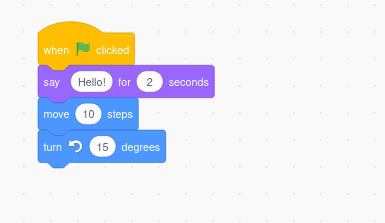
\includegraphics[scale=0.55]{img/scratch.png}
        \caption{Programa en Scratch}
        \label{figura:scratch}
\end{figure}

\subsection{Pensamiento computacional}
El pensamiento computacional es ``el proceso de pensamiento que interviene en la formulación de los problemas y sus soluciones, de manera que las soluciones se representen de forma que pueda ser realizada por un procesador de información''~\cite{wing2011research}. Para poder evaluar sus competencias se han definido los siguientes puntos basados en la herramienta Dr. Scratch:
\begin{enumerate}[1)]
    \item Paralelismo: sucesión simultánea de varias instrucciones o acciones. Por ejemplo, se necesitaría paralelismo si quisiésemos que dos personajes giren 15º a la vez.
    \item Condicionales: cuando las instrucciones se pueden ejecutar o no en función del resultado de una condición. Los condicionales más típicos, entre ellos, se incluyen los operadores lógicos (and, or, not).
    \item Control de flujo: hace referencia al orden en el que se ejecutan las instrucciones. El orden natural en un programa sería que la instrucciones fuesen ejecutándose una a una. Sin embargo, también se debe incluir la opción de ejecutar un conjunto de instrucciones hasta que suceda otro evento o que las instrucciones se ejecuten las veces que queramos (hablamos de bucles).
    \item Abstracción: se consigue dividiendo un problema grande en pequeños conjuntos más sencillos y simples separando en scripts o creando bloques definidos.
    \item Sincronización: supone el ajuste temporal de diferentes eventos. Es decir, cuando se desea ejecutar una instrucción una vez ha terminado otra se requiere que ambos eventos estén sincronizados.
    \item Interactividad con el usuario. Así, conseguimos hacer intervenir al usuario de alguna forma como puede ser introducir un nombre o pulsar una tecla.
    \item Datos: esto incluye las operaciones con las variables, listas y atributos.
    \item Diversidad: supone el uso de distintos tipos de bloques como de movimiento y de evento.
\end{enumerate}

\section{Snap! Berkeley}

Es una plataforma virtual que se programó en JavaScript como extensión de la ya mencionada plataforma Scratch. ~Snap! define un lenguaje de programación visual que permite programar por bloques. Como novedades implementa listas avanzadas y permite crear bloques definidos  más potentes. La página principal de Snap! se observa en la figura~\ref{figura:ppal_snap} y en ella podemos ver que nos ofrece la opción de correr el programa, de ver ejemplos y de obtener el manual de referencia. En Snap! Berkeley, además de crear programas, se pueden subir estos proyectos a la comunidad de Snap! para que todo el mundo pueda probarlos y ver cómo se han implementado.
\begin{figure}[h]
        \centering
        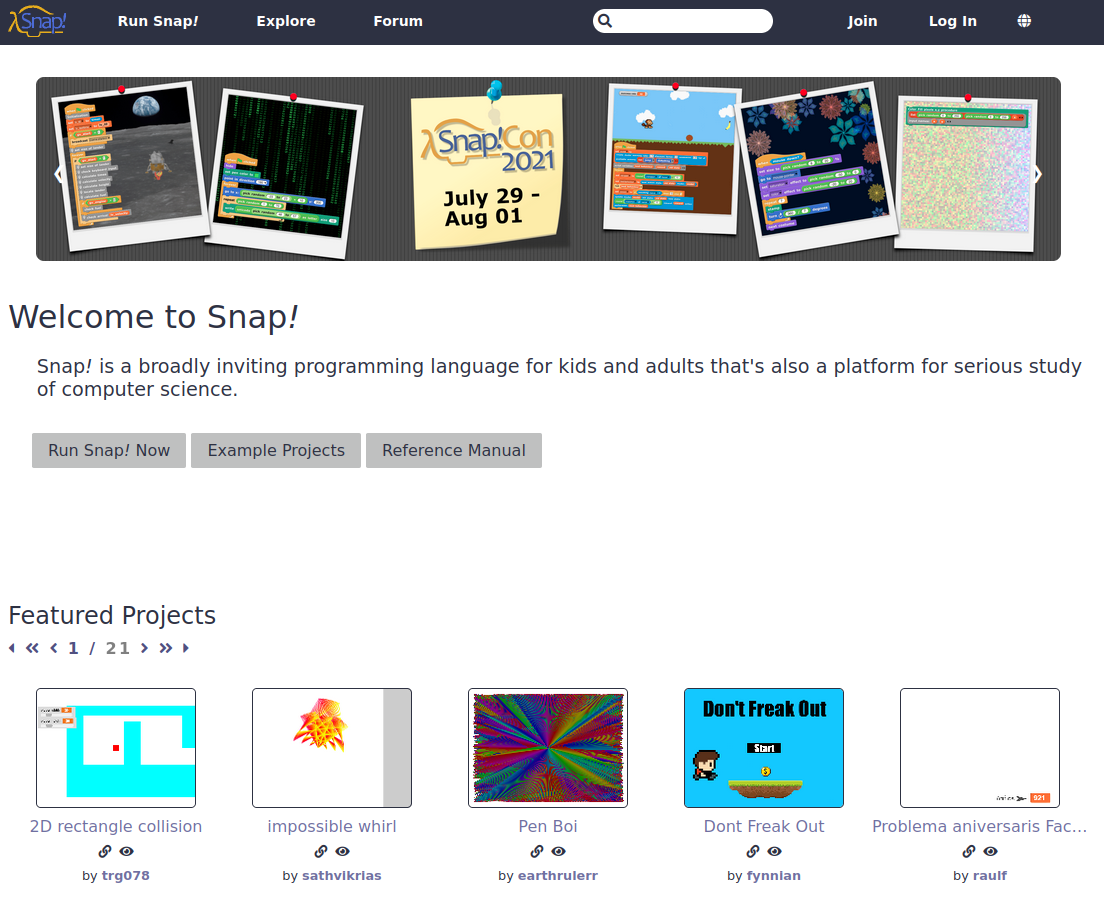
\includegraphics[scale=0.4]{img/snap_ppal.png}
        \caption{Página principal de Snap! Berkeley}
        \label{figura:ppal_snap}
\end{figure}


El manual de referencia consta de 11 capítulos y de 2 anexos y en ellos se explica en detalle todo lo relacionado con el manejo de sus bloques para programar. Por ejemplo, el capítulo I sección A trata sobre cómo crear paralelismo en Snap! gracias a la configuración de un tipo de bloques o el capítulo III te explica cómo crear tus propios bloques definidos.

El entorno de programación de Snap! donde se crean los programas se indica en la figura~\ref{figura:entorno_snapp}. En la sección indicada como A) se encuentran los bloques definidos de 8 categorías para crear los programas, la sección B) es donde se crean los conjuntos de instrucciones arrastrando los bloques y  uniéndolos entre ellos. Por último, la sección C) es donde se puede ver dichas instrucciones ejecutándose y siendo aplicadas a los personajes que definimos.
\begin{figure}[h]
        \centering
        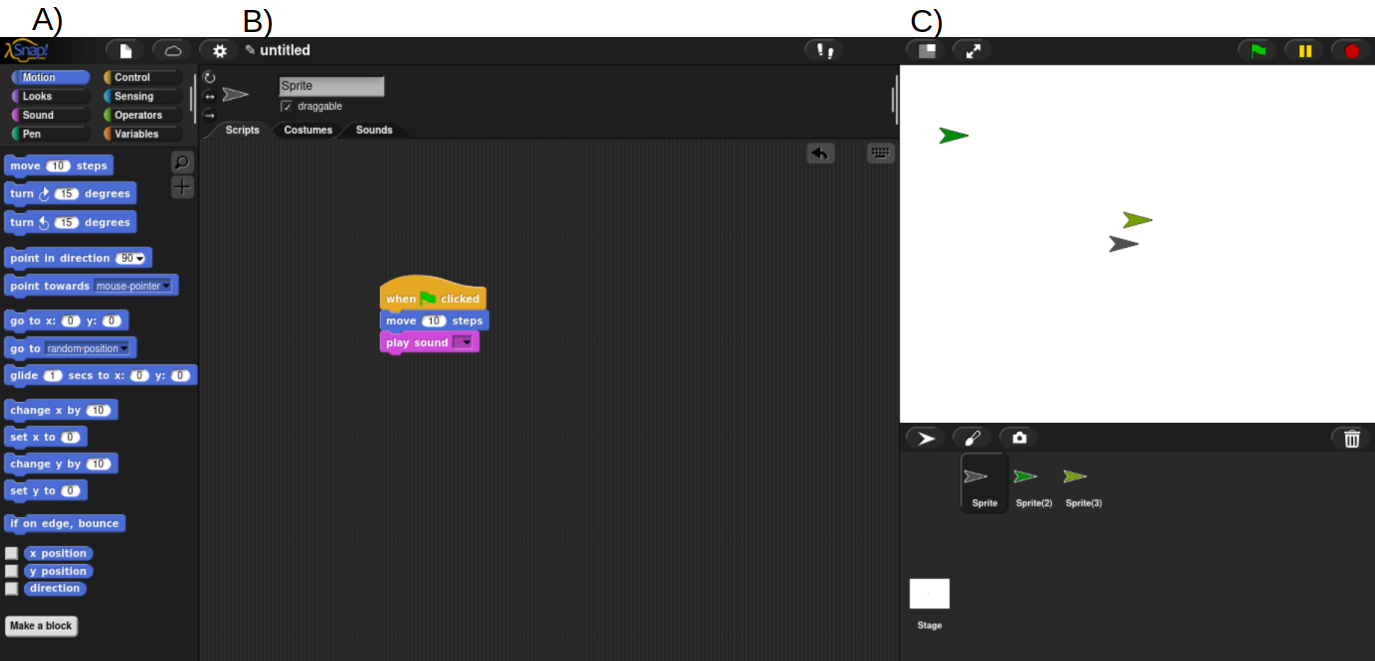
\includegraphics[scale=0.35]{img/entorno.png}
        \caption{Entorno para programar en Snap!}
        \label{figura:entorno_snapp}
\end{figure}
%%%%%%%%%%%%%%%%%%%%%%%%%%%%%%%%%%%%%%%%%%%%%%%%%%%%%%%%%%%%%%%%%%%%%%%%%%%%%%%%
%%%%%%%%%%%%%%%%%%%%%%%%%%%%%%%%%%%%%%%%%%%%%%%%%%%%%%%%%%%%%%%%%%%%%%%%%%%%%%%%
% OBJETIVOS %
%%%%%%%%%%%%%%%%%%%%%%%%%%%%%%%%%%%%%%%%%%%%%%%%%%%%%%%%%%%%%%%%%%%%%%%%%%%%%%%%

\cleardoublepage % empezamos en página impar
\chapter{Objetivos} % título del capítulo (se muestra)
\label{chap:objetivos} % identificador del capítulo (no se muestra, es para poder referenciarlo)

\section{Objetivo general} % título de sección (se muestra)
\label{sec:objetivo-general} % identificador de sección (no se muestra, es para poder referenciarla)

Mi trabajo fin de grado consiste en crear  una herramienta docente que analiza los proyectos creados en Snap! Berkeley, una implementación que permite programar de forma interactiva a partir de bloques. Para ello se ha creado una aplicación web a través del framework Django y con el servidor pythonanywhere.

\section{Objetivos específicos}
\label{sec:objetivos-especificos}

Para este proyecto hemos definido dos modos de interactuar:
\begin{itemize}
\item 
El modo estudiante  consiste en  analizar un fichero XML obtenido a través de la url del proyecto de Snap! El análisis está basado según una rúbrica  que lo divide en 8 secciones, admitiendo una calificación del 0 al 3 cada una.
\begin{itemize}
      \item
     Paralelismo
      \item
     Condicionales
      \item
      Control de flujo
      \item
      Abstracción
      \item
      Sincronización
      \item
      Interactividad
      \item
      Representación de datos
      \item
      Uso de categorías o diversidad
    \end{itemize}
El nivel final, que es el que da la calificación total del proyecto obtenida a partir de la media de todas sus partes, resulta ser:
    \begin{itemize}
          \item
          Nulo $\rightarrow $ [0, 0.5)
          \item
          Básico $\rightarrow $ [0.5, 1.5)
          \item
          Intermedio $\rightarrow $ [1.5, 2.5)
          \item
          Avanzado $\rightarrow $ [2.5, 3]
     \end{itemize}
\item
El modo profesor amplía el modo estudiante con la posibilidad de analizar un archivo ZIP en el que se encuentran los xml de los proyectos de sus alumnos. Una vez analizado todos los archivos XML, se da la opción de descargar las puntuaciones  de las 8 secciones y el nivel final en formato CSV.

\end{itemize}
Por último, para ambos modos se han definido varios dashboards en el que se muestran gráficos de los datos de los proyectos analizados.
\section{Planificación temporal}
\label{sec:planificacion-temporal}

A mí me gusta que aquí pongáis una descripción de lo que os ha llevado realizar el trabajo.
Hay gente que añade un diagrama de GANTT.
Lo importante es que quede claro cuánto tiempo llevas (tiempo natural, p.ej., 6 meses) y a qué nivel de esfuerzo (p.ej., principalmente los fines de semana).


%%%%%%%%%%%%%%%%%%%%%%%%%%%%%%%%%%%%%%%%%%%%%%%%%%%%%%%%%%%%%%%%%%%%%%%%%%%%%%%%
%%%%%%%%%%%%%%%%%%%%%%%%%%%%%%%%%%%%%%%%%%%%%%%%%%%%%%%%%%%%%%%%%%%%%%%%%%%%%%%%
% ESTADO DEL ARTE %
%%%%%%%%%%%%%%%%%%%%%%%%%%%%%%%%%%%%%%%%%%%%%%%%%%%%%%%%%%%%%%%%%%%%%%%%%%%%%%%%

\cleardoublepage
\chapter{Estado del arte}
\label{chap:estado}

En este apartado se explicará de forma breve y concisa los lenguajes de programación, bases de datos, modelos, arquitecturas y demás tecnologías que se hayan necesitado para la implementación de nuestra aplicación web.

\section{Snap! Berkeley}
Para entender el funcionamiento de Snap! es necesario definir algunos conceptos básicos de la programación por bloques~\cite{harvey2017snap}:
\begin{itemize}
    
    \item Block: existen diferentes clasificaciones. \begin{enumerate}[1)]
        \item Según las categorías:
   
            \begin{enumerate}[a)]
                \item Motion: bloques que permiten dar movimiento al sprite o personaje.
                \item Looks: permite cambiar las propiedades de apariencia del personaje.
                \item Sound: permite añadir sonidos, cambiar el volumen...
                \item Pen: permite pintar líneas o crear estampas del sprite.
                \\
                    \begin{figure}[h]
                        \centering
                        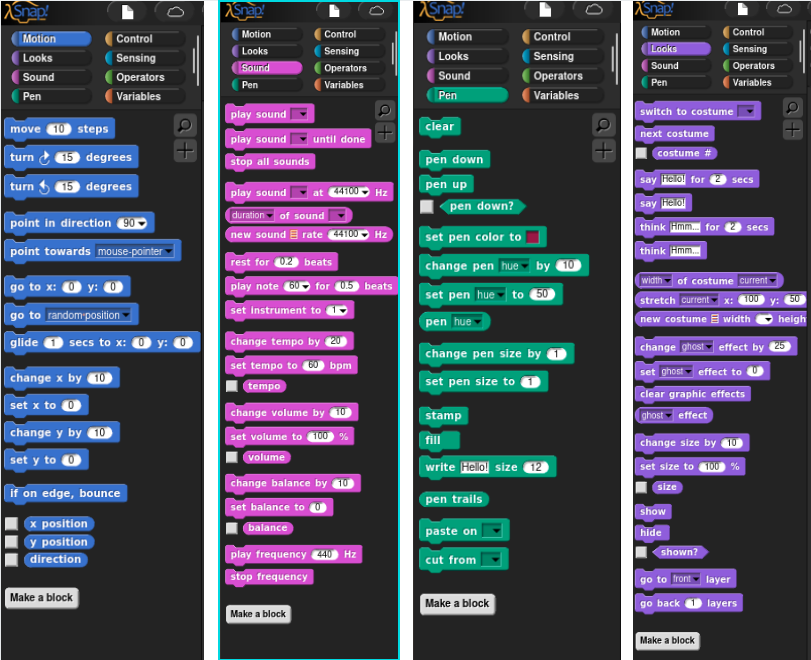
\includegraphics[scale=0.45]{img/4-blocks.png}
                        \caption{Bloques de tipo motion, look sound y pen respectivamente.}
                        \label{figura:bloque1}
                    \end{figure}
                \item Control: bloques para inicializar los scripts o para hacer bucles.
                \item Sensing: permite distinguir interacciones como cuando pulsas una tecla o cuando tocas un borde con el ratón.
                \item Operators: permite hacer operaciones como sumas, multiplicaciones,operaciones lógicas...
                \item Variables: incluye listas, operaciones con listas, inicialización de variables...
                \begin{figure}[h]
                        \centering
                        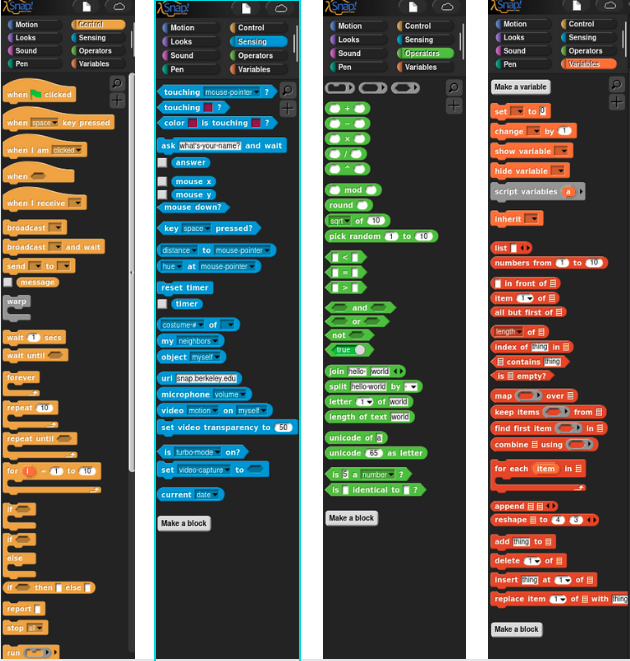
\includegraphics[scale=0.5]{img/blo4-2.png}
                        \caption{Bloques de tipo motion, lookm sound y pen respectivamente.}
                        \label{figura:bloque2}
                \end{figure}
                 \end{enumerate}
        \item Según su funcionalidad:
            \begin{enumerate}[a)]
             \item Command block: se corresponden con bloques que tienen acciones ya definidas.
             \item Reporter block: proporciona un valor de entrada que será usada en una acción.
             \item Predicate: es otro tipo de ``reporter block'' ya que devuelve una entrada de tipo True o False. Tiene sentido usarlos en bucles o condicionales.
            \end{enumerate}
        \item Según su forma:
             \begin{enumerate}[a)]
             \item Hat block: son los que se usan para inicializar un script y solo se pueden poner al principio.
             \item Brick shape: de forma simple y de tipo command block.
             \item C shape: es de tipo command pero admite dentro de él otro script o un único brick shape. Se corresponde con los bucles y los condicionales.
             \item E shape: compuesto con dos bloques C shape.
             \item Oval shape: se corresponde con los reporter block. Por ejemplos, las variables son óvalos de color naranja.
             \item Hex shape: se corresponde con los predicate block.
             \end{enumerate}
        En la figura~\ref{figura:shape} tenemos varios ejemplos.
        
        \begin{figure}[h]
                        \centering
                        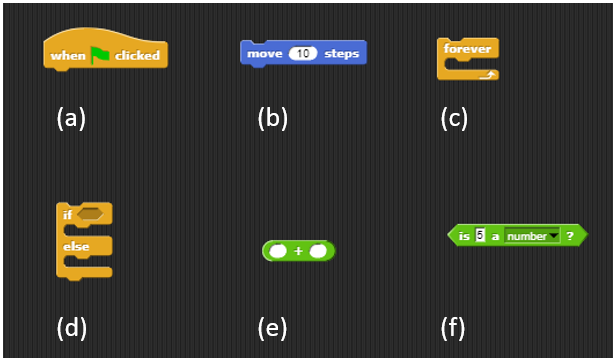
\includegraphics[scale=0.55]{img/shapes.PNG}
                        \caption{Bloques según la forma en Snap!}
                        \label{figura:shape}
        \end{figure}
    \end{enumerate}


    \item Script: es una pila o agrupación de bloques que se inicializan con los hat blocks y realizan un conjunto de acciones como en la figura~\ref{figura:script}.

     \begin{figure}[h]
        \centering
        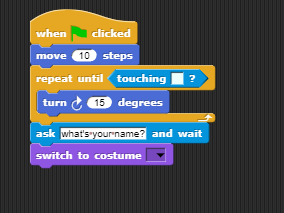
\includegraphics[scale=1]{img/script.PNG}
        \caption{Script en Snap!}
        \label{figura:script}
    \end{figure}
    
    \item Sprite: Hace referencia a los diferentes gráficos o personajes de nuestro programa. Por ejemplo, en la figura~\ref{figura:sprites} se puede observar que tenemos dos sprites (cuadrado y círculo) y a cada uno de ellos se les pueden asignar funciones de movimiento, sonidos, es decir, cada sprite tiene sus propios scripts. 
    \begin{figure}[h]
        \centering
        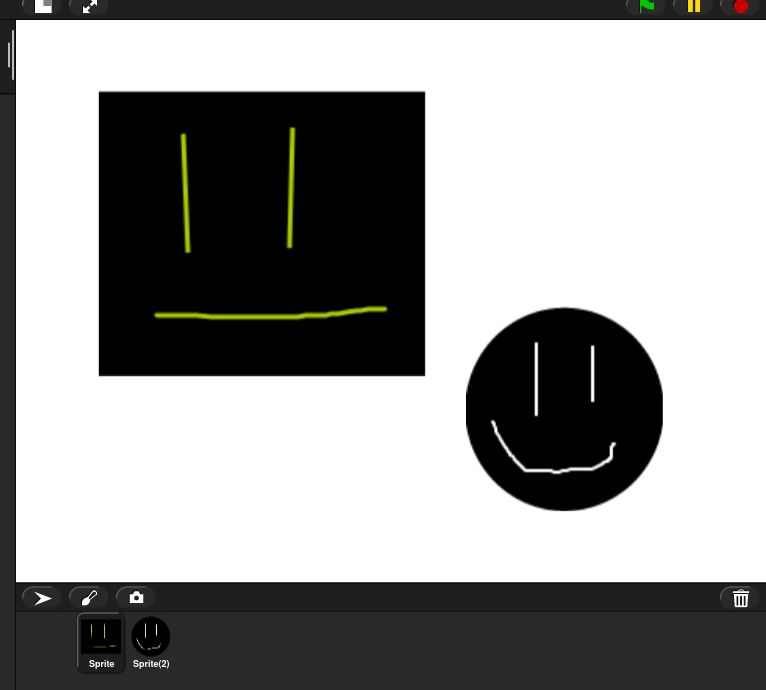
\includegraphics[scale=0.2]{img/sprite.png}
        \caption{Dos sprites en snap!}
        \label{figura:sprites}
    \end{figure}
\end{itemize}

\section{Modelo cliente-servidor} 
\label{sec:seccion1}
A día de hoy, la mayoría de las aplicaciones utilizan un esquema basado en el llamado modelo cliente-servidor. Es una arquitectura orientada a servicios donde los clientes son los usuarios de los servicios y de sus servidores asociados~\cite{castro2015arquitectura}.
 \begin{itemize}
          \item
         Cliente: es la parte encargada de mandar peticiones al servidor y recibir las respuestas de este. Los usuarios interaccionan con la parte del cliente.
          \item
          Servidor: es la parte encargada de ofrecer un servicio, es decir, de recibir peticiones por parte de los clientes y de proveerles las respuestas adecuadas a dichas peticiones.~\cite{lizama2016redes} 
     \end{itemize}
     
Las ventajas de este modelo:
\begin{itemize}
    \item Centralizado
    \item Mantenimiento simple
    \item Da servicios a más de un cliente 
    \item Interoperabilidad con el uso de protocolos estándar
\end{itemize}

Las desventajas de este modelo:
\begin{itemize}
    \item Problemas de congestión directamente proporcional al número de clientes
    \item Mantenimiento simple
    \item Escalable~\cite{lizama2016redes} 
\end{itemize}

\begin{figure}[h]
        \centering
        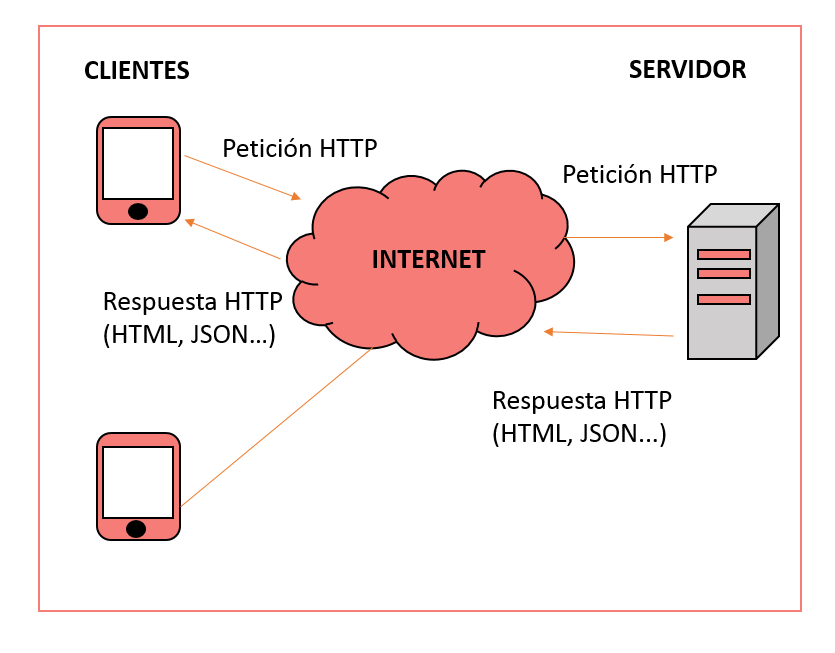
\includegraphics[scale=0.4]{img/Cliente-Servidor.png}
        \caption{Modelo cliente servidor}
        \label{figura:cliente-servidor}
    \end{figure}

Cabe mencionar que es un modelo de aplicación distribuida ya que las tareas que se realizan (solicitar recursos o enviarlos) se reparten entre cliente y servidor. Por tanto, distinguimos 3 partes fundamentales de una aplicación distribuida:
\begin{itemize}
    \item Capa de presentación: también llamada interfaz de usuario, es responsable del control de la interacción entre el usuario y la aplicación. Se engloban todas las tareas que deben ser realizadas por la parte cliente del modelo general~\cite{marini2012modelo}. Por ejemplo, para el aspecto de la aplicación web se puede usar CSS, un lenguaje de estilos. Además,esta capa se corresponde en la actualidad con el concepto de \textit{frontend} de una aplicación web.
    \item Capa de negocio: es la capa intermedia ya que se comunica con la capa de presentación y con la capa de datos.~\cite{bazurto2018arquitectura} Asegura las directrices o reglas del negocio, controla las secuencias de acciones y aísla los cambios de las interfaces de los usuarios y de los datos.~\cite{marini2012modelo} 
    \item Capa de datos: es la que tiene los datos y la que se encarga de acceder a ellos y operar con ellos. Esta capa se corresponde con el concepto de \textit{backend}. Las tecnologías que se incluyen en esta capa son tales como los gestores de bases de datos o los frameworks.
\end{itemize}
\begin{figure}[h]
        \centering
        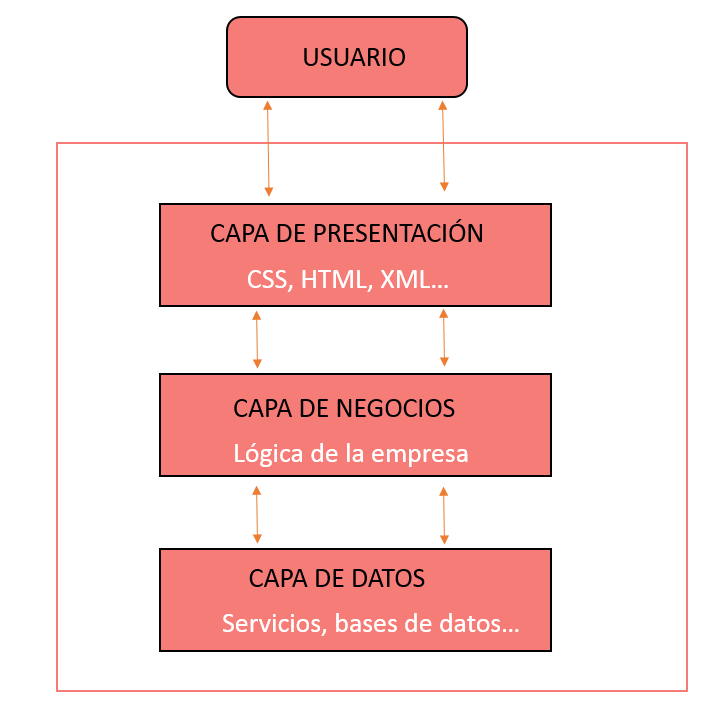
\includegraphics[scale=0.4]{img/3capas.png}
        \caption{Modelo de 3 capas}
        \label{figura:3capas}
\end{figure}
\section{Arquitectura MVC y Django}
La arquitectura MVC divide las partes de una aplicación en modelo, vista y controlador de forma que se pueda implementar cada parte por separado. Al ser entidades independientes, el cambio de una de ellas no supondrá la necesidad de cambiar ninguna de las otras~\cite{gonzalez2012patron}. Django es el framework que usamos para esta aplicación y se basa en este patrón MVC:

\begin{itemize}
    \item Modelo: se encarga de la representación de los datos. En Django se corresponde con el módulo models.py.
    \item Vista: se corresponde a la lógica de aplicación y se encarga de la presentación al usuario de los datos del modelo. En Django, las vistas se corresponden al módulo views.py y delegan la presentación de información en las plantillas o templates. Por eso, se puede decir que su arquitectura es MTV (modelo-template-vista) en vez de MVC como podemos observar en la figura~\ref{figura:MVC}.
    \item Controlador: recibe los eventos de entrada y contiene reglas de gestión de eventos como indicar cambios al modelo o elegir la vista adecuada para mostrar resultados. 
\end{itemize}

\begin{figure}[h]
        \centering
        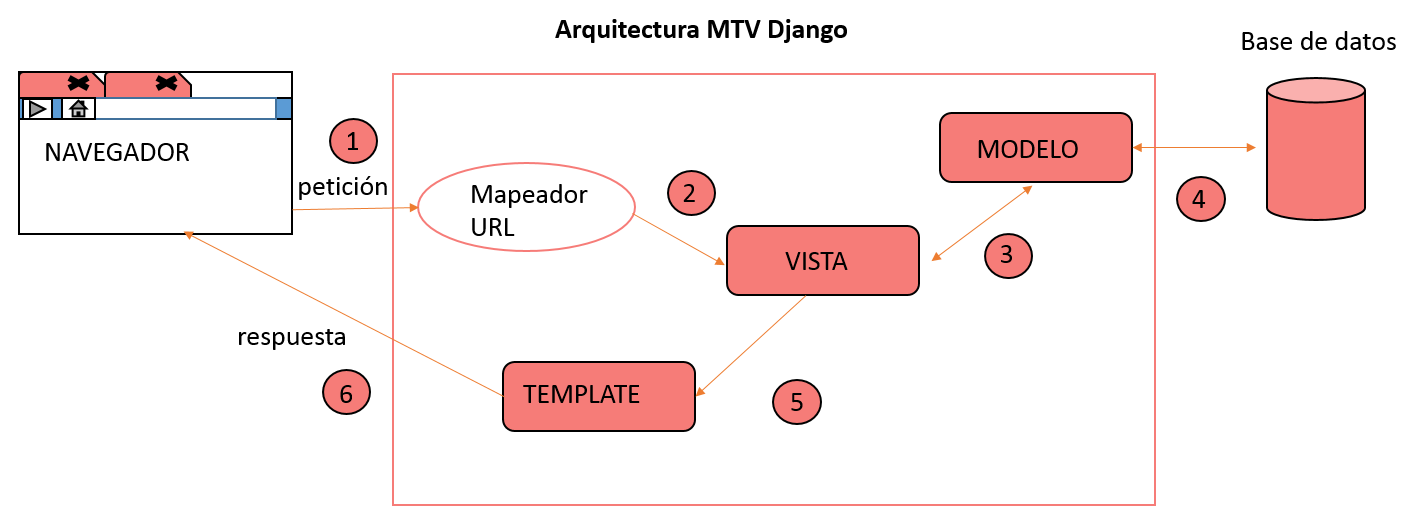
\includegraphics[scale=0.4]{img/django_request.png}
        \caption{Arquitectura MVC en Django}
        \label{figura:MVC}
\end{figure}
\section{Representational state transfer}
REST es un modelo de diseño de servicio web que define un conjunto de principios de una arquitectura basada en recursos apto únicamente para aplicaciones distribuidas. Supone una mejora en la facilitación en el intercambio  de  datos  entre  el  cliente  y  el  servidor  que, por ejemplo, el protocolo simple de acceso a objetos (SOAP).  Sus principios son:
\begin{enumerate}[a)] % (a), (b), (c), ...
\item Modelo cliente (capa de presentación) - servidor (capa de negocio y datos) sin estado. No es necesario recordar ningún dato ya que las peticiones HTTP que se generan llevan incluidas todas las cabeceras y datos necesarios para dar una respuesta sin depender del estado anterior.
\item Estructura URI para los recursos.
\item Transferencia de hipermedios como XML o JSON para la representación de datos o de estado de los recursos.
\item Uso de métodos HTTP y principio CRUD (create, read, update and delete). Por tanto, las operaciones que afectan a un recurso pueden ser:
\begin{itemize}
    \item GET: petición para obtener un recurso.
    \item POST: petición para crear un recurso en el servidor.
    \item PUT: petición para actualizar un recurso en el servidor.
    \item DELETE: petición para eliminar un recurso.~\cite{rodriguez2008restful}
\end{itemize}
\end{enumerate}
\section{FRONTEND}
Para la interfaz de usuario o la capa de presentación hemos utilizado en nuestro diseño web diferentes tecnologías como son HTML, CSS y JavaScript.
\begin{figure}[h]
        \centering
        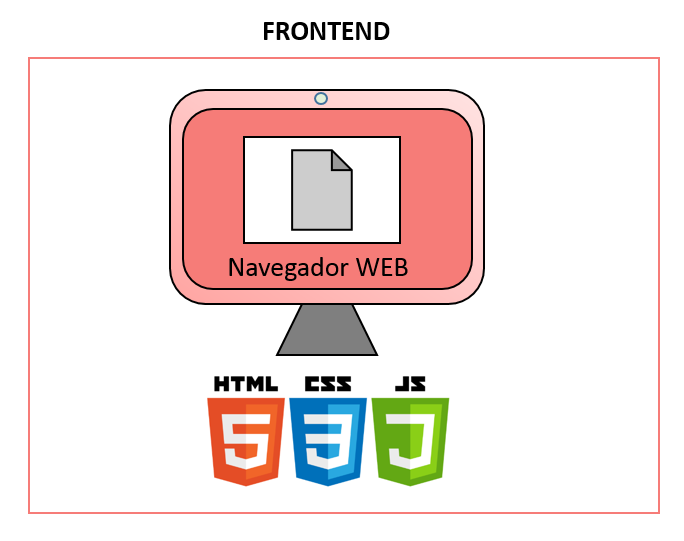
\includegraphics[scale=0.4]{img/frontend.png}
        \caption{Elementos FRONTEND}
        \label{figura:frontend}
\end{figure}
\subsection{HTML}
HyperText Markup Language, en español lenguaje marcado de hipervínculos, es el lenguaje básico de construcción de páginas web. Se basa en texto que contiene referencias a enlaces, imágenes, tablas, textos u otros elementos. Un elemento HTML debe ir entre etiquetas que definen la orden o instrucción de lo que se quiere insertar~\cite{equipo2009diseno}.Por ejemplo, para insertar un título se podría usar la etiqueta h1 o para insertar una imagen img. HTML se encarga de crear el contenido de la página web pero no del estilo o apariencia de dicha página, para ello es necesario el CSS. 

\begin{figure}[h]
        \centering
        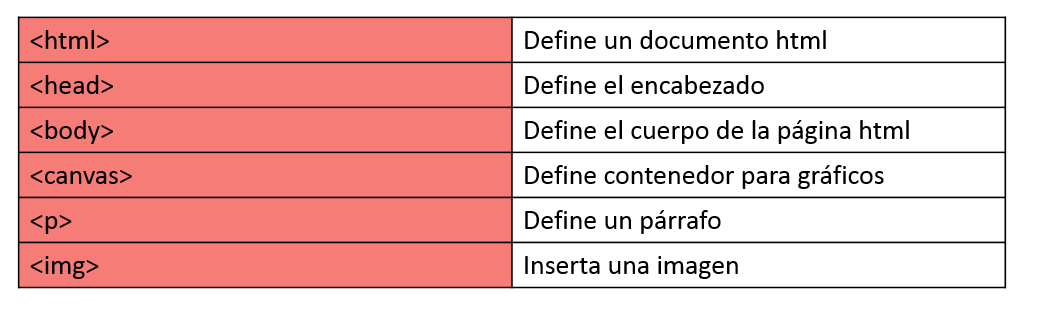
\includegraphics[scale=0.6]{img/tags.PNG}
        \caption{Etiquetas en HTML}
        \label{figura:tags}
\end{figure}
\subsection{CSS}
Cascading Style Sheets, en español hojas de estilo en cascada, es el lenguaje de estilos que permite modificar la apariencia de páginas webs construidas en HTML. La sintaxis de una instrucción CSS es una declaración que tiene una propiedad y un valor~\cite{mdn}. La propiedad es la característica de estilo que se quiere cambiar, por ejemplo si queremos cambiar el fondo la propiedad sería ``background'', y el valor sería el color o imagen del fondo que se querría cambiar. Se agrupan las declaraciones referidas a un elemento concreto de HTML, denominado selector, en un bloque. En la figura~\ref{figura:css} se muestra un ejemplo de CSS dando estilo a un código HTML.

\begin{figure}[h]
        \centering
        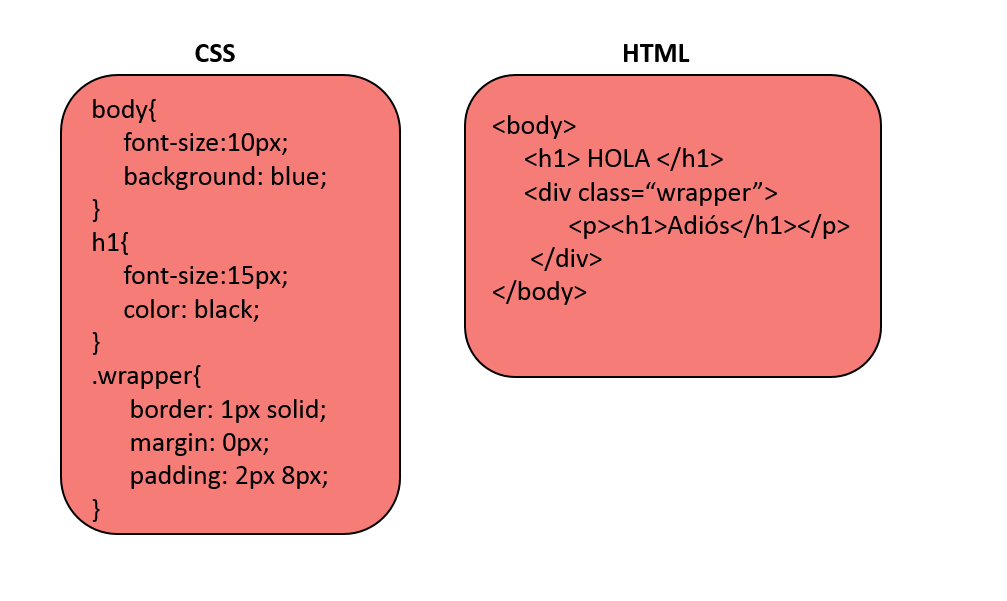
\includegraphics[scale=0.4]{img/cssyhtml.PNG}
        \caption{CSS asociado al HTML}
        \label{figura:css}
\end{figure}
\subsection{JavaScript}
Lenguaje de programación interpretado y orientado a objetos usado para crear contenido dinámico en las páginas webs. Para insertar código JS en HTML se debe indicar con la etiqueta script.  Ofrece la oportunidad de convertir una página web que en un principio era estática, en una página interactiva donde se pueda incluir menús emergentes, botones para hacer click o incluso animaciones~\cite{mdn1}. Esto es posible gracias al modelo de programación basada en eventos utilizado por JavaScript en el que el script espera a que el usuario interactúe de alguna forma (evento), procesa la información y responde con una acción a través de una función. Por ejemplo, cuando el usuario pincha la pantalla el evento se denomina onClick. Cada evento tiene asociada una función que ejecuta JavaScript denominada ´´event handler''~\cite{perez2019introduccion}.

\section{BACKEND}
Se corresponde con la parte del servidor, la base de datos y la aplicación. Para ello utilizamos un lenguaje de programación (en nuestro caso Python), un framework para desarrollar el sitio web (Django), una base de datos (sqlite3) y un proveedor de  servidor  online donde lanzar la aplicación (pythonanywhere). En la figura~\ref{figura:backend} vemos distintas tecnologías que forman parte del \textit{backend}.
\begin{figure}[h]
        \centering
        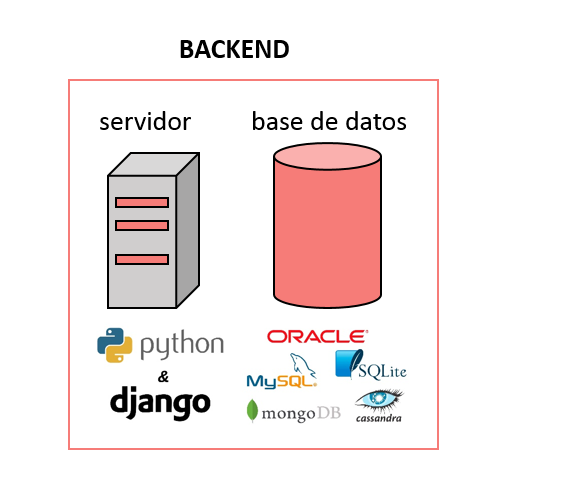
\includegraphics[scale=0.6]{img/backend.png}
        \caption{BACKEND}
        \label{figura:backend}
\end{figure}
\subsection{Pyhton}
Lenguaje de programación creado por Guido van Rossum en los 90, administrado por Python Software Foundation y con licencia de código abierto. En nuestra aplicación web usaremos la versión 3.8.5. Las caracterísicas principales de este lenguaje son las siguientes~\cite{gonzalez2014python}:
\begin{itemize}
    \item Lenguaje de alto nivel e interpretado
    \item Tipado dinámico 
    \item Fuertemente tipado
    \item Multiplataforma
    \item Programación orientada a objetos aunque permite también la programación imperativa, funcional y programación orientada a aspectos.
\end{itemize}
\subsection{Django}
Es un framework de alto nivel que permite crear una aplicación web usando python de forma sencilla cuyas características más destacadas son~\cite{bennett2009practical}:
\begin{itemize}
    \item Tiene un mapeador objeto relacional (ORM) que es una librería que reconoce y relaciona cómo es la base de datos o el código que tú escribas.
    \item Conjunto de librerías HTTP que gestionan las peticiones y respuestas.
    \item Libería de ruta de urls para localizar el código que corresponde a la URL introducida. 
    \item Sistema de plantillas que conforman la interfaz del usuario.
    \item Basado en el patrón MVC con la variación de que las vistas delegan la presentación al sistema de plantillas.
    \item Por defecto la base de datos es sqlite3 pero se puede usar otras como MySql, PostgreSQL u Oracle configurándolo en el módulo settings.py.
   
\end{itemize}

\begin{figure}[h]
        \centering
        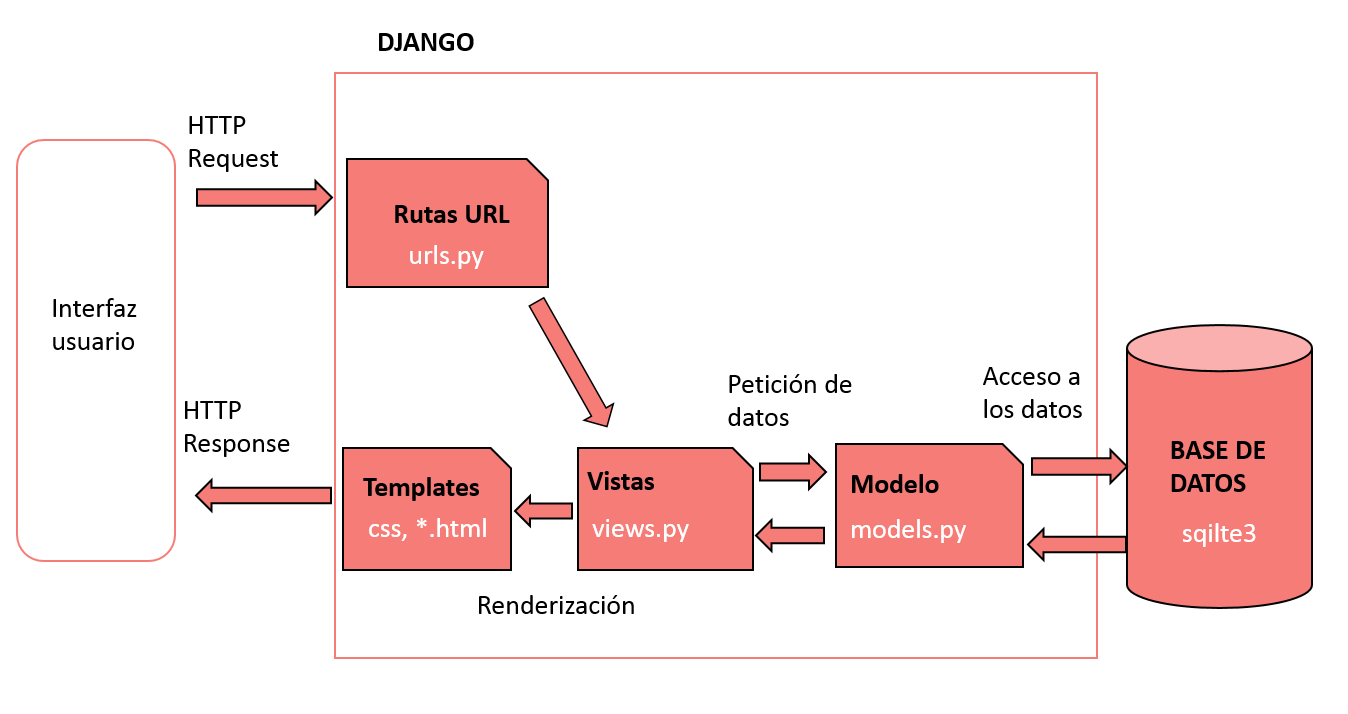
\includegraphics[scale=0.5]{img/django.png}
        \caption{Aplicación en Django }
        \label{figura:appDjango}
\end{figure}
\subsection{SQLite3}
SQLite es un motor de datos SQL mundialmente utilizado, este motor está desarrollado en una biblioteca programada en C la cual tiene compatibilidad con la mayoría de lenguajes de programación utilizados a día de hoy, SQLite es un motor SQL confiable dado que la mayoría del código fuente presente en su biblioteca está destinado a la realización de test unitarios y procesos de validación, cabe destacar en SQLite las siguientes características~\cite{sqlite}: 
\begin{itemize}
    \item Autónomo y cuasi independiente: En el proceso de ejecución no existe un uso de más recursos que los proporcionados en el código fuente de SQLite, no realizando así un uso de bibliotecas u programas externos del sistema.
\item Carencia de servidor: Para este motor el sistema cliente-servidor clásico es cosa del pasado, pudiendo permitir que el proceso que requiera de SQLite lea y escriba directamente desde los archivos de la base de datos en disco. 
\item Configuración Cero: A diferencia de aplicaciones u otras tipologías de bases de datos, SQLite opta por la configuración cero, en la cual no es necesario configurar nada ni definir ningún parámetro para indicar a nuestro sistema que SQLite está presente. En la biblioteca no podremos encontrar ficheros de configuración.
\item Base de Datos transaccional: Esta dinámica aporta seguridad y estabilidad al proceso de la base de datos, en caso de una avería del sistema o de un corte de energía durante la transacción con un registro de la base de datos, SQLite detiene o confirma la transacción de forma automática, evitando de esta forma transacciones incompletas o fallos en el proceso.

\end{itemize}
\subsection{PythonAnywhere}
Proporciona un servidor  para poder subir tu aplicación web a la nube. Es compatible con proyectos de Django y existen dos modalidades: de pago y gratuita. La de pago tiene más ventajas y opciones como es la posibilidad de elegir el dominio, al contrario que, la versión gratuita que te impone el dominio \url{http://yourusername.pythonanywhere.com/}. En nuestro caso, la aplicación estará alojada en \url{http://prodriguezmartinez.pythonanywhere.com/}.


%%%%%%%%%%%%%%%%%%%%%%%%%%%%%%%%%%%%%%%%%%%%%%%%%%%%%%%%%%%%%%%%%%%%%%%%%%%%%%%%
%%%%%%%%%%%%%%%%%%%%%%%%%%%%%%%%%%%%%%%%%%%%%%%%%%%%%%%%%%%%%%%%%%%%%%%%%%%%%%%%
% DISEÑO E IMPLEMENTACIÓN %
%%%%%%%%%%%%%%%%%%%%%%%%%%%%%%%%%%%%%%%%%%%%%%%%%%%%%%%%%%%%%%%%%%%%%%%%%%%%%%%%

\cleardoublepage
\chapter{Diseño e implementación}
En este capítulo detallaremos cómo hemos trabajado con las tecnologías explicadas en el capítulo 3 para poder crear la aplicación Dr. Snap!
\section{Arquitectura general} 
La arquitectura de la aplicación creada la podemos dividir como se muestra en la figura~\ref{figura:esquema}.
\begin{figure}[h]
            \centering
            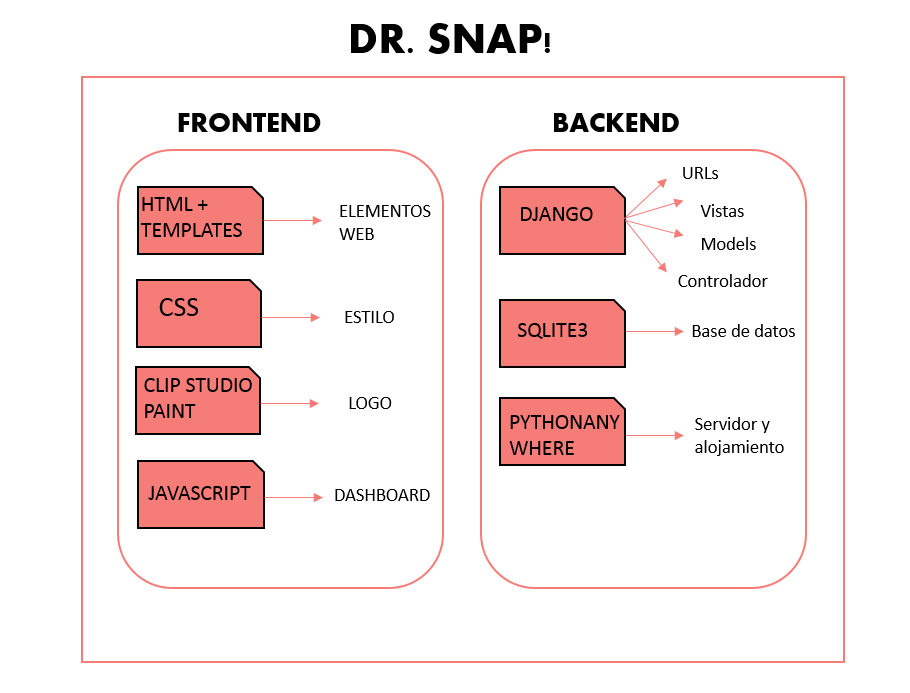
\includegraphics[scale=0.5]{img/arquitectura.PNG}
            \caption{Esquema global de la aplicación.}
            \label{figura:esquema}
        \end{figure}

\label{sec:arquitectura}
\subsection{FRONTEND}
En este apartado se desarrolla la capa de presentación o interfaz del usuario. Para el aspecto de la aplicaciń web hemos añadido un estilo CSS asociado a unas plantillas HTML (templates) y hemos diseñado un logo con el programa Clip Studio Paint.
\begin{enumerate}[a)]
    \item \textbf{HTML Y TEMPLATES}:
    
    Las plantillas definen los elementos HTML de la página web en conjunto con el CSS que se encarga de dar el estilo y apariencia de los elementos de las plantillas. En este proyecto se ha usado una plantilla de referencia gratuita que se puede encontrar en el enlace siguiente. Se han hecho los cambios pertinentes para quedar de la forma que aparece en la figura~\ref{figura:index} donde se define la cabecera, el menú horizontal, el logo y el pie de página.\\
    
     \begin{figure}[h]
            \centering
            
\includegraphics[scale=0.32]{img/index.png}
            \caption{Página índice de Dr. Snap!}
            \label{figura:index}
        \end{figure}
    
    A raíz de esta template ``índice'' se han extendido las demás gracias a las funcionalidades de Django``built-in template'' y ``template inheritance'' que permiten dejar bloques sin definir los cuales las plantillas ``hijo''  que se creen serán las encargadas de rellenarlos. Estas heredan los elementos de la de referencia como es la cabecera o el menú principal. De esta forma, se evita repetir código. En la figura~\ref{figura:herencia} se muestra el funcionamiento de la herencia de plantillas de Django en Dr. Snap! donde index.html es la plantilla de referencia y *.html, las plantillas hijo que dan contenido al bloque cuerpo heredando todos los demás elementos de index.html.
    
        \begin{figure}[h]
            \centering
            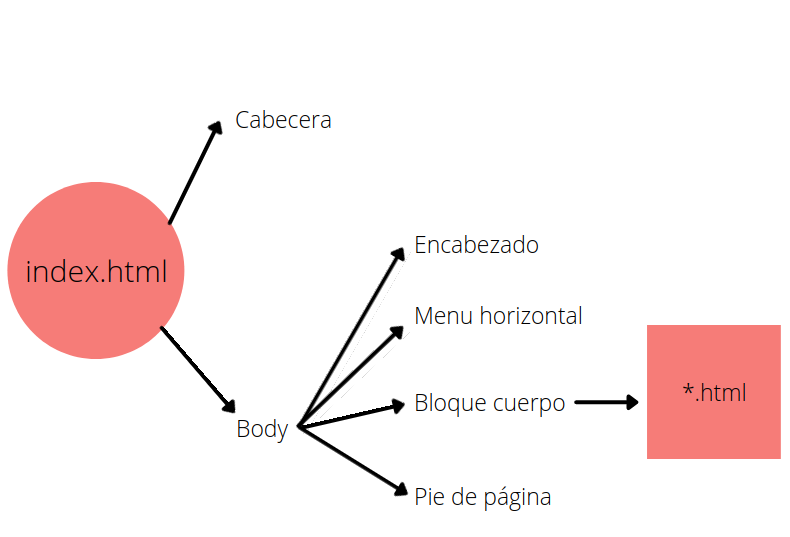
\includegraphics[scale=0.33]{img/herencia.png}
            \caption{Templates inherit en Django}
            \label{figura:herencia}
        \end{figure}
        
    Así resulta un directorio de plantillas para nuestra aplicación web como en la figura~\ref{figura:template} donde cada una de ellas se cargará con el contenido adecuado según las peticiones que reciba el servidor de Django o las respuestas que proporcione. Esto se consigue gracias a la función de renderizado que nos provee el framework Django y que se explicará más adelante en la parte de \textit{backend}.\\
      \begin{figure}[h]
            \centering
            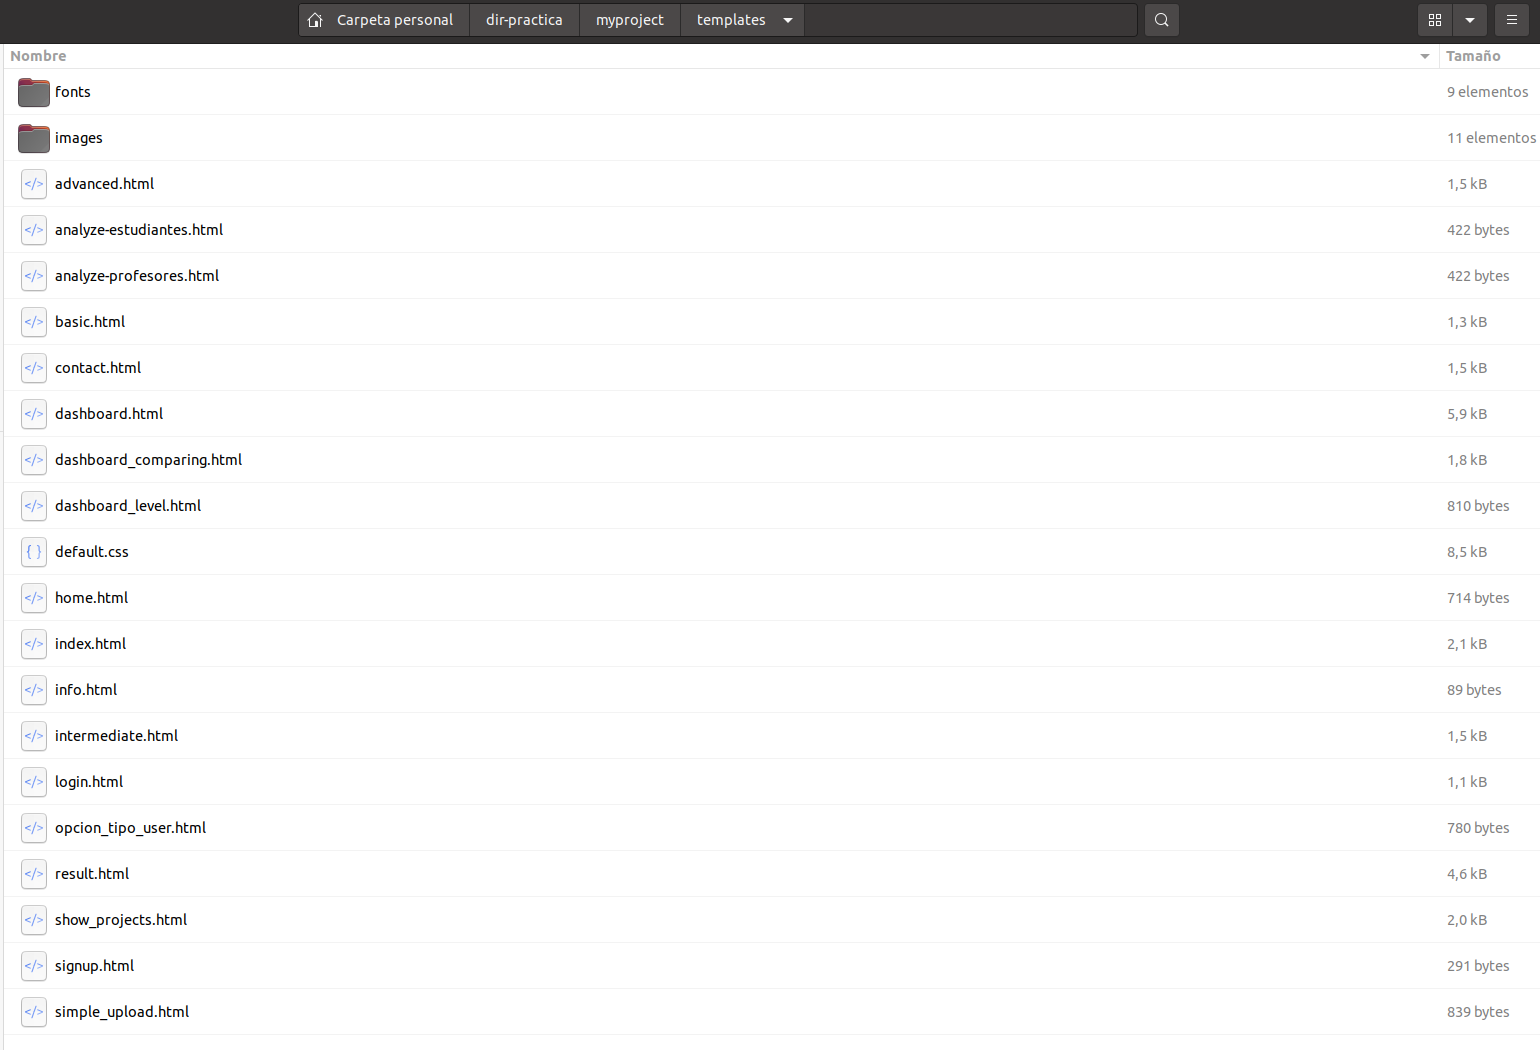
\includegraphics[scale=0.245]{img/plantillas.png}
            \caption{Directorio de templates de Dr. Snap!}
            \label{figura:template}
        \end{figure}
    \item \textbf{CSS}:
    
    Como ya explicamos, el CSS es un lenguaje de estilo que proporciona las propiedades de apariencia de los elementos definidos en las plantillas HTML. Por ejemplo, en la figura~\ref{figura:cssyhtml} vemos como se vería la página sin CSS y con CSS. 
    \\
    \begin{figure}[h]
            \centering
            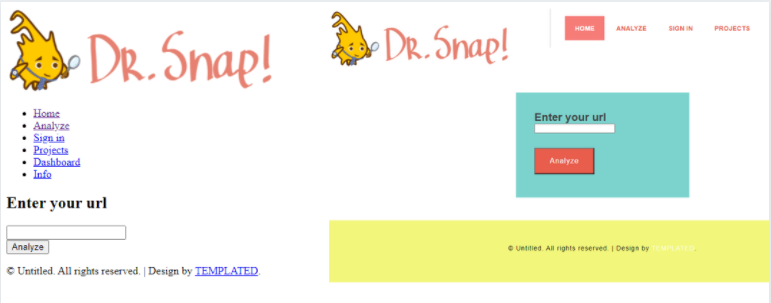
\includegraphics[scale=0.75]{img/css_2.PNG}
            \caption{ Página web sin CSS y con CSS}
            \label{figura:cssyhtml}
        \end{figure}
    
    Así, para dar estilo al botón de analyze del formulario lo definiríamos en CSS como aparece en la figura~\ref{figura:boton}, donde se hace referencia al elemento button (etiqueta en HTML) y se escriben las propiedades que queremos que tenga como es el color, el tamaño o la letra.\\
    
      \begin{figure}[h]
            \centering
            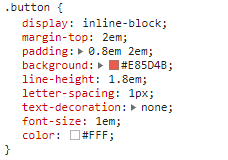
\includegraphics[scale=1.5]{img/css_boton.PNG}
            \caption{Código CSS de un botón}
            \label{figura:boton}
        \end{figure}
    
    
    \item \textbf{CLIP STUDIO PAINT PRO}:
    
    Programa de ilustración digital que se ha utilizado para diseñar el logo y algunas imágenes. Para este programa se ha requerido el conocimiento básico de diseño de viñetas, aplicación de tonos y texturas y del manejo de diferentes capas. Para el logo me he basado en el muñeco original de Snap! y le he añadido unas gafas, cejas, una corbata, un reloj y una lupa para darle un toque de profesor. En la figura~\ref{figura:logos} se puede ver la comparación de ambos. 
    \\
        \begin{figure}[h]
            \centering
            
\includegraphics[scale=0.4]{img/logos.png}
            \caption{Muñeco de Snap! y de Dr. Snap!}
            \label{figura:logos}
        \end{figure}
        
    Además del logo y el muñeco, se ha cambiado la imagen principal de Snap! Berkeley añadiendo el lema de \textit{analyze your own project} en vez de \textit{build your own project} y cambiando al muñeco de Dr. Snap!. Se hizo gracias al sistema de capas que permite borrar zonas y añadir nuevas y se puede ver en la imagen~\ref{figura:snap}.
    
    \begin{figure}[h]
            \centering
            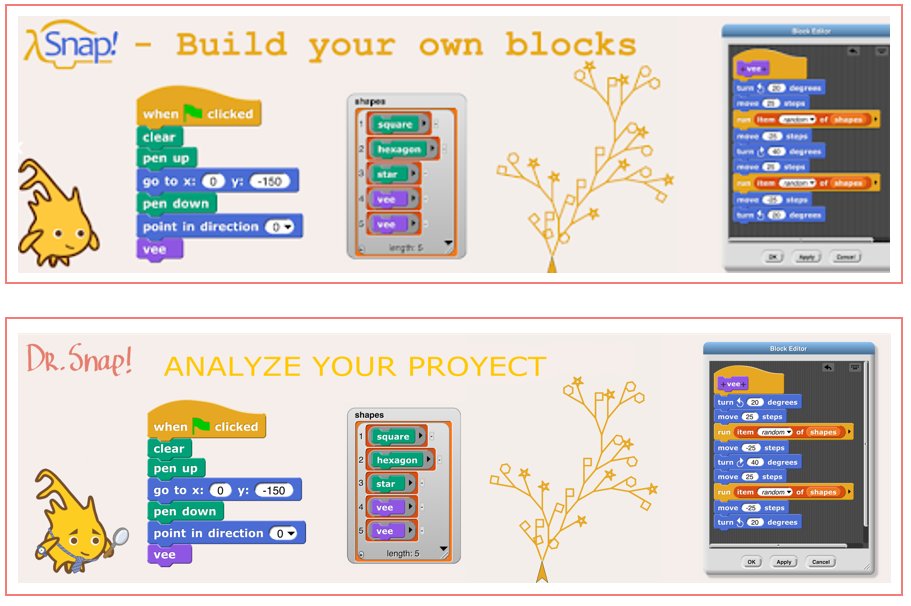
\includegraphics[scale=0.35]{img/snap.PNG}
            \caption{Imagen principal aplicación web Dr. Snap!}
            \label{figura:snap}
        \end{figure}
        
     Por último, para expresar los niveles de cada proyecto se me ocurrió poner al muñeco con un bocadillo de texto diciendo el nivel del proyecto. Los 4 niveles se observan en la figura~\ref{figura:levels}.
     
    \begin{figure}[h]
            \centering
            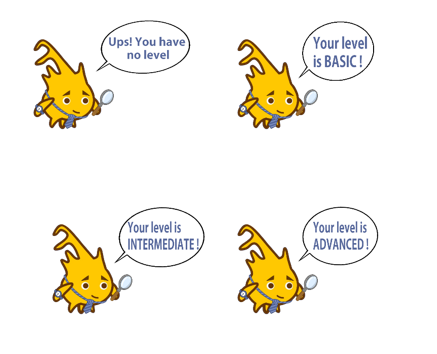
\includegraphics[scale=0.8]{img/levels.PNG}
            \caption{Imagen que dice el nivel de un proyecto.}
            \label{figura:levels}
        \end{figure}
    
    
    \item \textbf{JAVASCRIPT}:
    
       Se ha usado JavaScript para implementar un conjunto de dashboards. Un dashboard es un gráfico que muestra datos en forma de gráficos (diagrama de barras, de línea o donuts, por ejemplo) y con ello ver un resumen de los datos para poder estudiarlos y analizar posibles tendencias . En esta aplicación se han desarrollado tres de ellos gracias a javascript y a su librería de código abierto Chart.js que admite 8 tipos de gráficos (de línea, de barra, de donut, circular, burbuja, radar, polar y de dispersión) y es responsive, adapta su diseño para la mejor visualización posible según el dispositivo desde el que se vea. De los tipos que proporciona hemos seleccionado el gráfico de barras y el gráfico de donut. Esta librería, además de implementar dichos gráficos, permite la configuración y la interacción con ellos. Por ejemplo, se puede cambiar los colores de los gráficos, poner nombres a cada eje, añadir animaciones o gestionar todo tipo de eventos. En la figura~\ref{figura:js} se observa un gráfico circular y un gráfico de líneas. 
    \begin{figure}[h]
            \centering
            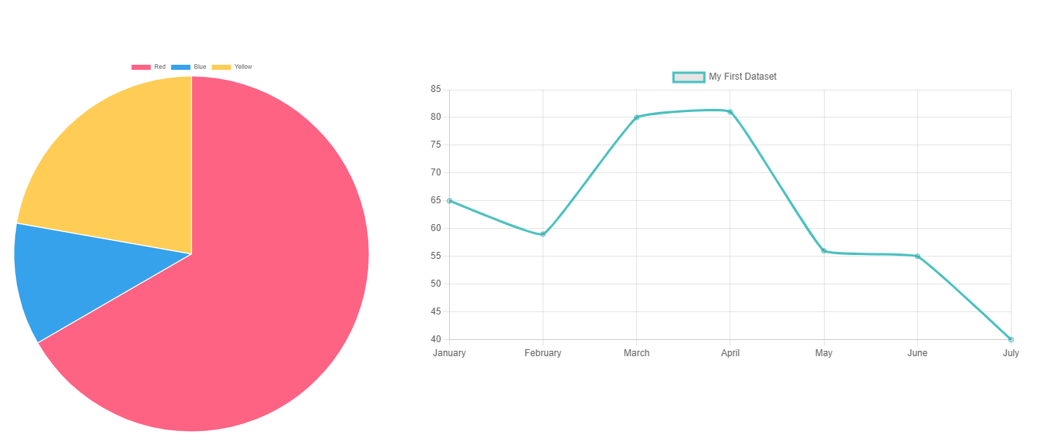
\includegraphics[scale=0.5]{img/chart.PNG}
            \caption{Gráfico circular y de líneas respectivamente de Chart.js}
            \label{figura:js}
        \end{figure}
    
       
\end{enumerate}

\subsection{BACKEND}
\begin{enumerate} [a)]
    \item \textbf{DJANGO:}
    
    Hemos descargado Django versión 3.1.1 y Python 3.8.5 para el desarrollo de la aplicación web. Como hemos mencionado Django será el entorno que nos permitirá crear la aplicación web de una forma muy sencilla. 
    
    Cuando nos creamos una aplicación en Django, lo primero que tenemos que hacer es configurar los diferentes módulos que hay. En la figura~\ref{figura:carpetas} podemos ver una representación de las carpetas y módulos más importantes que hay en un proyecto de Django: la carpeta llamada ``myproject'' contiene todos los módulos y archivos que gestionan el proyecto, la carpeta de nombre ``myfirstapp'' contiene todos los módulos y archivos que gestionan la aplicación web, el archivo ``db.sqlite3'' es la base de datos, la carpeta ``media'' es la que contiene todos los zips que los profesores suben, la carpeta ``template'' es en la que se guardan todas las plantillas HTML y el archivo ``manage.py'' es el manejador que se ejecuta, por ejemplo, para lanzar la aplicación o para crear nuevas migraciones.
     \begin{figure}[h]
            \centering
            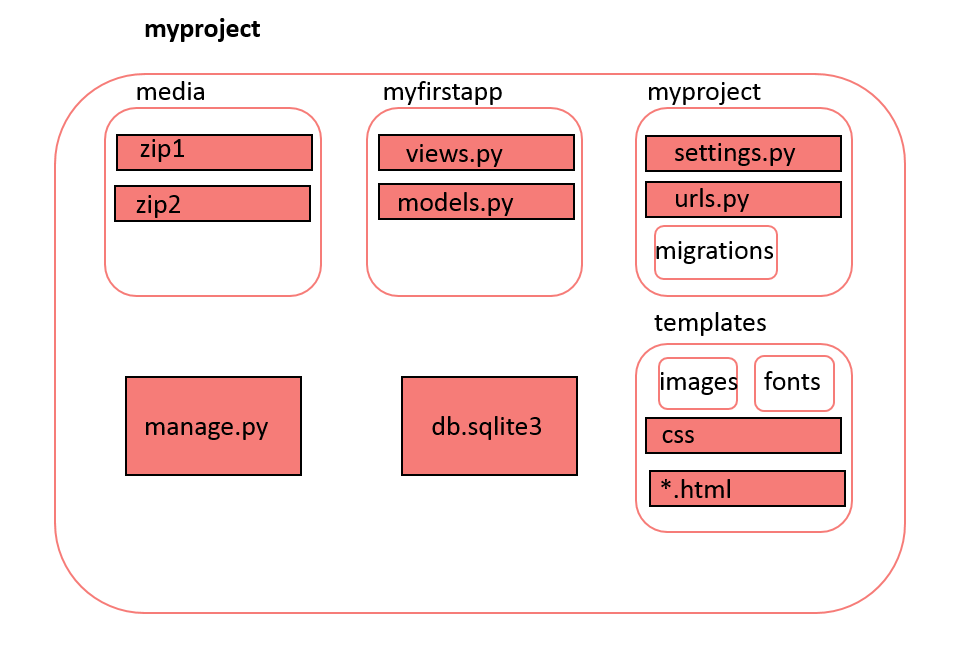
\includegraphics[scale=0.6]{img/carpetas.PNG}
            \caption{Principal directorio del proyecto en Django.}
            \label{figura:carpetas}
        \end{figure}
        
    Veamos los módulos más importantes con mayor profundidad:
    \begin{itemize}
        \item settings.py: se debe configurar el nombre de la aplicación que has creado, los servidores que están permitidos, como es en nuestro caso \textit{pythonanywhere} o \textit{mylocalhost}; todos los paths o rutas donde encontrar los archivos estáticos, las plantillas u otros; la base de datos que queremos utilizar (por defecto, utiliza sqlite3) e incluso hay que configurar datos como la zona horaria o el idioma.
        \item urls.py: en este módulo definimos las posibles urls que vamos a encontrar en nuestra aplicación web y especificamos la vista asociada a dicho path url. En la tabla~\ref{Tabla:paths} podemos ver un resumen de las distintas urls que hemos definido con su vista asociada y la funcionalidad que tienen.
        
        \begin{table}[]
        \centering
            \begin{tabular}{|l|l|l|}
            \hline
            PATH URL & VISTA & FUNCIÓN \\ \hline
            / & principal & Proporciona la página principal de la aplicación \\ \hline
            /contact & info & Página que da información sobre la aplicación \\ \hline
            /analyze & analyze & \begin{tabular}[c]{@{}l@{}}Página que permite analizar los proyectos o \\ zips según el modo en el que estés.\end{tabular} \\ \hline
            /basic & basic & Informa sobre los criterios para nivel básico. \\ \hline
            /intermediate & intermediate & Informa sobre los criterios para nivel intermedio. \\ \hline
            /advanced & advanced & Informa sobre los criterios para nivel avanzado. \\ \hline
            /login & login\_user & Permite iniciar sesión. \\ \hline
            /type-signup & choose & \begin{tabular}[c]{@{}l@{}}Permite registarse eligiendo si eres estudiante o \\ profesor.\end{tabular} \\ \hline
            /signup & signup & Permite registrarse. \\ \hline
            /logout & logout\_user & Permite cerrar sesión. \\ \hline
            /projects & show\_projects & \begin{tabular}[c]{@{}l@{}}Permite ver los proyectos analizados o introducir \\ un zip para descargarse el proyecto en csv.\end{tabular} \\ \hline
            /project/\textless{}name\textgreater{} & show\_project & \begin{tabular}[c]{@{}l@{}}Permite ver las puntuaciones de un proyecto y\\ su nivel.\end{tabular} \\ \hline
            /dashboard & dashboard & \begin{tabular}[c]{@{}l@{}}Enseña los gráficos con los proyectos por nivel\\ y da la opción de ver los de un zip o la \\ comparación de dos zips.\end{tabular} \\ \hline
            /dashboard/\textless{}tag\textgreater{} & dashboard\_level & \begin{tabular}[c]{@{}l@{}}Permite ver  los proyectos al hacer un\\ click en uno de los niveles de los dashboard.\end{tabular} \\ \hline
            /admin/ & admin.site.urls & Gestiona los usuarios y contraseñas, entre otras. \\ \hline
            \end{tabular}
            \caption{Paths admitidos con sus vistas asociadas de Django.}
            \label{Tabla:paths}
        \end{table}
        
        
        
        \item views.py: son las funciones que reciben una petición HTTP, deben devolver una respuesta HTTP y están asociadas a un path de url como hemos explicado anteriormente. El ORM de Django recibe un path con una petición, mapea en el listado de urls a qué vista corresponde y se ejecuta dicha función para devolver la respuesta correcta renderizada con una de las plantillas HTML. Es decir, por ejemplo, si hacemos desde el navegador una petición GET para el recurso /analyze, la función vista analyze nos devolverá la respuesta HTTP definida en la función renderizada con la plantilla que hicimos para dicho recurso. La figura~\ref{figura:MVC} resume lo explicado. También se pueden hacer redirecciones a otras páginas, en caso de error mostrar página 404 o, incluso, pasar datos a las plantillas.
        \item models.py: se definen las clases  y sus respectivos campos para la base de datos. En nuestra aplicación web tendremos tres clases: usuario, proyectos y el tipo de usuario (profesor o estudiante). En la figura~\ref{figura:models} queda reflejado las tres clases y sus campos correspondientes. Cabe destacar que la clase user ya viene implementada por el sistema de autenticación de usuarios de Django (en ``django.contrib.auth''), el cual proporciona funciones como login, logout o signup o la clase \textit{models.user}.
           \begin{figure}[h]
            \centering
            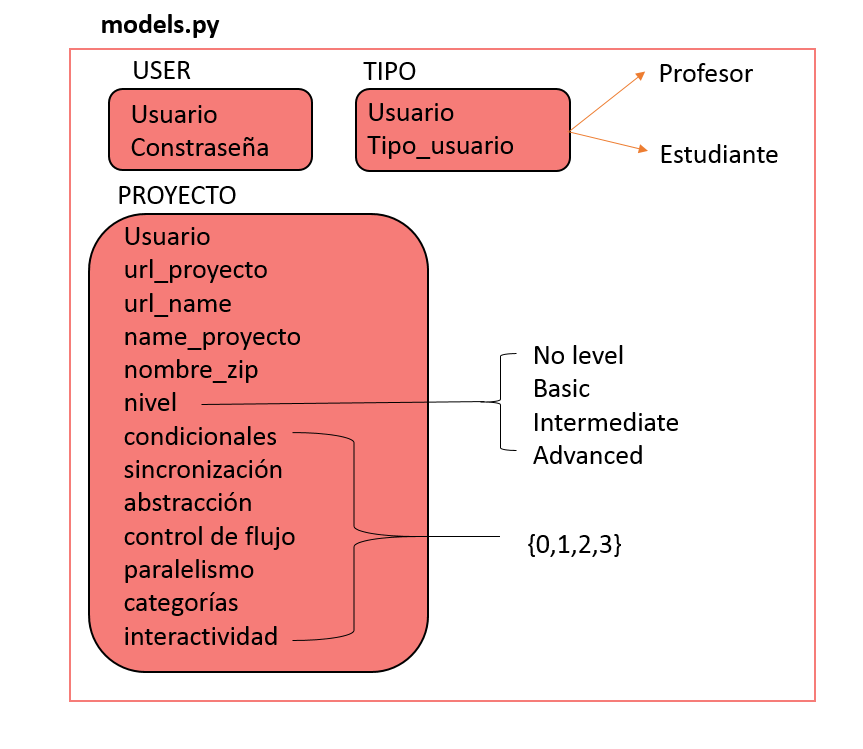
\includegraphics[scale=0.45]{img/models.PNG}
            \caption{Clases y campos definidos en models.py}
            \label{figura:models}
        \end{figure}
    \end{itemize}
    
    \item \textbf{SQLITE3:}
    
    Como hemos dicho previamente, nuestra base de datos será la que viene por defecto en Django, es decir, sqlite3. Es una base de datos sencilla y para crearla lo primero que debemos es indicarla en settings.py. Una vez definidas las clases en models.py se debe hacer una migración con los cambios hechos para luego migrarla. Cada vez que se cree una clase, se añada un campo nuevo o se elimine se debe hacer una migración que refleje estos cambios y luego migrarla a la base de datos.  En la figura~\ref{figura:bbdd} se observan todas las tablas que hay creadas, sin embargo, las únicas que hemos creado nosotros, gracias al módulo de models.py, son las que empiezan por el nombre de la aplicación, es decir, \textit{myfirstapp\_proyectos} y \textit{myfirstapp\_tipo}. Todas las demás son implementadas por Django para diferentes funcionalidades, por ejemplo, \textit{auth user} es la tabla que representa la ya comentada clase user que viene ya predefinida con los campos de contraseña, gmail, primer apellido...\\
    
       \begin{figure}[h]
            \centering
            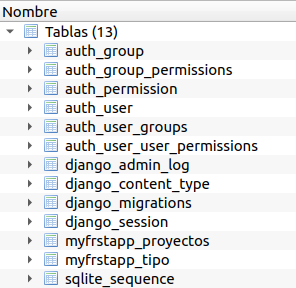
\includegraphics[scale=0.55]{img/bbdd.png}
            \caption{Tablas de la base de datos de la aplicación}
            \label{figura:bbdd}
        \end{figure}
    
    \item \textbf{PYTHONANYWHERE:}
    
    Para lanzar la aplicación de Django en pythonanywhere lo primero que debes hacer es crearte una cuenta de forma gratuita y clonar tu proyecto que debe estar previamente subido a github. El siguiente paso es crearte un entorno virtual y descargar Django. Hay que configurar los paths del directorio donde está el código, las templates y los recursos estáticos. Una vez hecho todo esto ya tenemos disponible nuestra aplicación web durante 3 meses, en nuestro caso,  en  http://prodriguezmartin.pythonanywhere.com
    
    Una vez que lancé la aplicación web al probarla tenía un error que impedía usarla: no dejaba hacer peticiones ni redirecciones a otros sitios webs a no ser que estos estuvieran en la \textit{whitelist} de pythonanywhere o que mi cuenta fuese de pago. Para solucionar el problema, me puse en contacto con los técnicos y conseguí, tras mucha insistencia, añadir el dominio de \url{https://cloud.snap.berkeley.edu/} a la \textit{whitelist} ya que me denegaron el dominio de https://snap.berkeley.edu/ lo que supuso algunos cambios mínimos en el código de la aplicación web.

\end{enumerate}

\section{Funcionalidades de Dr. Snap!}
En este apartado vamos a explicar todas las funciones que he implementado para que la aplicación web cumpla su cometido como herramienta docente. Estas siguen un orden cronológico ya que algunas han surgido con el objetivo de mejorar o complementar otras.
\subsection{Analizar proyectos}
Para analizar un proyecto se necesita la URL del proyecto de Snap! y así conseguir el XML donde viene guardada la información de bloques, scripts y sprites del proyecto. La URL se consigue a través de un formulario como el de la figura~\ref{figura:xml}. Una vez que tenemos la URL, se pensó que habría que interactuar con la API de Snap!, sin embargo, tras ver el código fuente descubrimos que no es necesario ya que existe una función implementada en JavaScript que te devuelve el XML simplemente haciendo un GET con el recurso /projects/user\_name/project\_name a Snap! Berkeley. 

En la figura~\ref{figura:xml} se ven los pasos necesarios para conseguir los datos de un proyecto de Snap! Berkeley: el usuario envía la URL de su proyecto a través de un POST, se parsea la URL, se forma la nueva URL y se hace una petición GET con esa URL a Snap! Berkeley; el cual, nos devuelve el XML correspondiente.

  \begin{figure}[h]
            \centering
            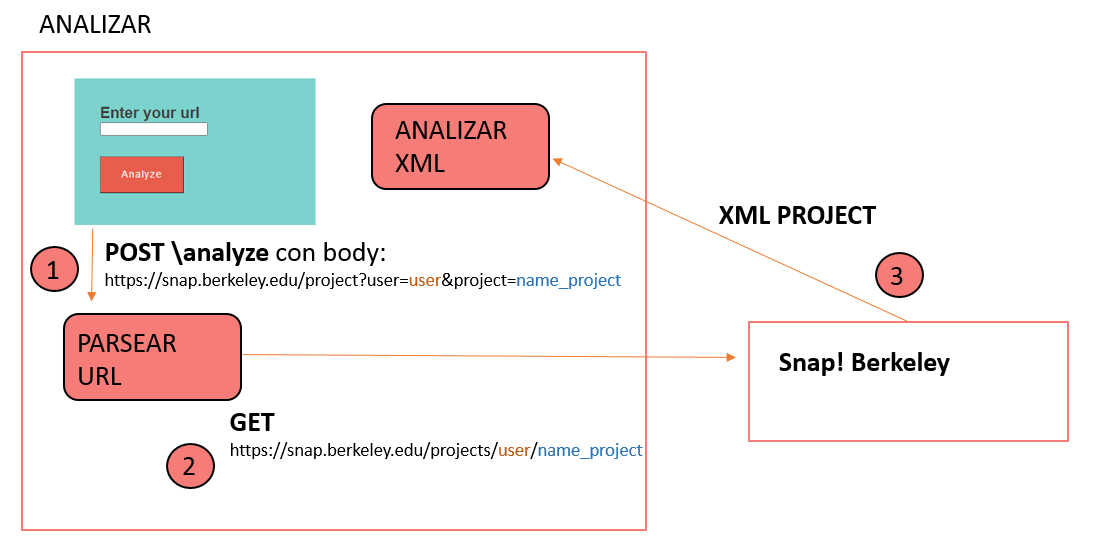
\includegraphics[scale=0.55]{img/analizar.PNG}
            \caption{Petición del XML de un proyecto}
            \label{figura:xml}
    \end{figure}
        
 Una vez que tenemos el XML tenemos que parsearlo para poder obtener todos los datos necesarios y, para ello, hemos hecho uso de la API xml.sax. Un archivo XML es un texto compuesto de etiquetas creado para formar una estructura de datos e información. Gracias al ContentHandler y al parser de xml.sax podemos acceder a cada etiqueta y a su contenido. Para ello, la clase ContentHandler define 3 funciones muy importantes:
 \begin{itemize}
     \item  def \_\_init\_\_ (self) en la que se deben inicializar todas las variables.
     \item def startElement (self, name, attrs) es la función que encuentra inicios de etiqueta XML, donde name se convierte en el nombre de la etiqueta y attrs en los atributos que hay en la etiqueta. Por ejemplo, block s=``move'' el nombre de la etiqueta es block, el atributo es s y su valor es move. En este punto guardaremos en un diccionario JSON los atributos y valores correspondientes  según necesitemos. Se ha tomado la decisión de trabajar con JSON porque es mucho más sencillo y rápido.
     \item def endElement(self, name) es la función que se encuentra con el cierre de etiquetas XML y sirve para saber que ya  has avanzado a otra etiqueta.

 \end{itemize}
 Para analizar un documento XML tenemos que:
 \begin{itemize}
     \item Crear un lector de XML con make\_parser().
     \item  Crear un manejador de contenido del XML con myContentHandler().
     \item Definir las funciones del ContentHandler y añadírselas al parser con setContentHandler(theHandler).
     \item Parsear la url donde se encuentra el archivo XML con el parser ya definido.
 \end{itemize}
Este paso puede que haya sido el más complicado de todos pues los proyectos de Snap! tienen una estructura XML más o menos similar pero no llega a ser única por lo que al intentar analizar las etiquetas resultó difícil porque no todos los proyectos encajaban con lo que había definido. En la figura~\ref{figura:tree} se refleja el esquema de etiquetas que se ha supuesto y cómo lo hemos guardado. Con esta estructura pretendemos poder guardar en un JSON solamente  los sprites que hay, los scripts y los bloques que se utilizan. Como extra se han guardado las variables y los bloques que puede crear un usuario. \\
El JSON se compone de 4 listas (sprites, variables, block-definition y name block-definition) que contienen diccionarios con sus datos. Por ejemplo, en sprites se guardan diccionarios por cada bloque parseado con los campos nº sprite, nº script, block y nº block.
\\
\begin{figure}[h]
\centering
            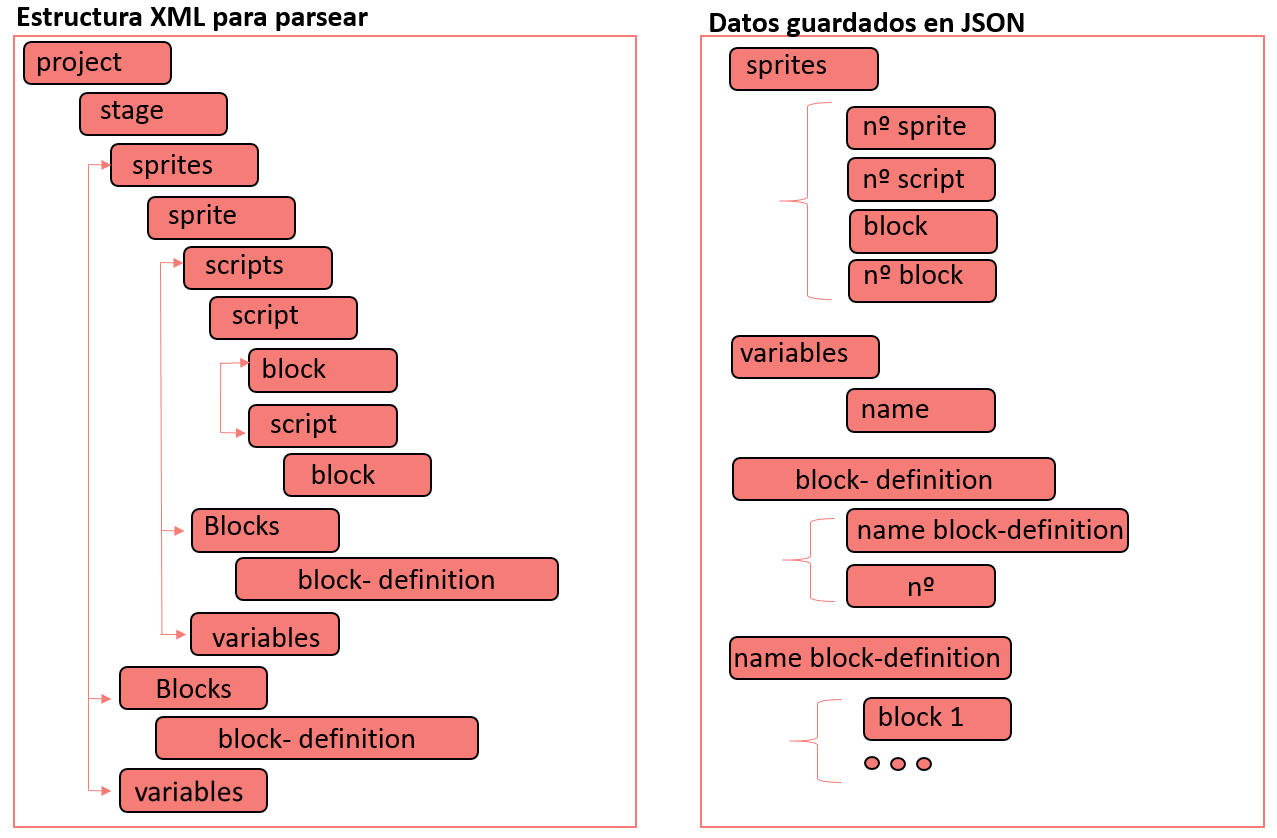
\includegraphics[scale=0.52]{img/tree_xml.PNG}
            \caption{Estructura seguida para parsear el XML y estructura seguida para guardar los datos parseados}
            \label{figura:tree}
    \end{figure}
    
Una vez que los datos se han guardado en el JSON, se procedió a implementar la rúbrica en Django con 7 categorías: paralelismo, abstracción, datos, flujo de control, diversidad o categorías, condicionales, sincronización e interactividad. Los criterios de evaluación quedan reflejados en la tabla y tienen de base la  de Dr. Scratch. Cada categoría tendrá, por tanto, una puntuación  Nula (0), Básica (1), Intermedia (2) o Avanzada (3), y para la puntuación global, se hará la media de las 8 categorías resultando una puntuación de: nivel nulo de 0 a 0.5, básico de 0.5 a 1.5, intermedio de 1.5 a 2.5 y avanzado de 2.5 a 3. Si el usuario ha iniciado sesión toda esta información se guarda en la base de datos en la tabla proyecto ya mencionada.
\begin{table}[h]
\centering
\begin{tabular}{l|l|l|l|}
\cline{2-4}
 & Básico & Intermedio & Avanzado \\ \hline
\multicolumn{1}{|l|}{Paralelismo} & \begin{tabular}[c]{@{}l@{}}1 sprite \& \textgreater{}= 2 scripts\\ receiveGo\\ receiveKey\end{tabular} & \begin{tabular}[c]{@{}l@{}}\textgreater{}= 2 sprites \& \textgreater{}= 1 script\\ receiveGo\\ receiveKey\end{tabular} & \begin{tabular}[c]{@{}l@{}}\textgreater{}=1 sprite \& 2 \textgreater{}= scripts\\ receiveCondition\\ receiveMessage\\ receiveOnClone\end{tabular} \\ \hline
\multicolumn{1}{|l|}{Condicionales} & Do if & \begin{tabular}[c]{@{}l@{}}DoIfElse\\ ReportIfElse\end{tabular} & \begin{tabular}[c]{@{}l@{}}ReportAnd\\ ReportOr\\ ReportNot\end{tabular} \\ \hline
\multicolumn{1}{|l|}{Control flujo} & \textgreater{}= 2 blocks en un script & \begin{tabular}[c]{@{}l@{}}DoForever\\ doRepeat\end{tabular} & \begin{tabular}[c]{@{}l@{}}DoUntil\\ for\end{tabular} \\ \hline
\multicolumn{1}{|l|}{Abstracción} & \textgreater{}=2 scripts & \textgreater{}=2 scripts, sprites & Definition-blocks \\ \hline
\multicolumn{1}{|l|}{Sincronización} & doWait & \begin{tabular}[c]{@{}l@{}}doBroadcast\\ receiveMessage\\ doStopThis\\ doPauseAll\end{tabular} & \begin{tabular}[c]{@{}l@{}}doWaitUntil\\ doBroadcastAndWait\\ receiveOnClone\\ receiveCondition\end{tabular} \\ \hline
\multicolumn{1}{|l|}{Interactividad} & \begin{tabular}[c]{@{}l@{}}receiveGo\\ receiveKey\end{tabular} & \begin{tabular}[c]{@{}l@{}}receiveInteraction\\ reportTouchingObject\\ reportKeyPressed\end{tabular} & \begin{tabular}[c]{@{}l@{}}doAsk\\ video\\ audio\end{tabular} \\ \hline
\multicolumn{1}{|l|}{Datos} & Atributos de los personajes & Operaciones con variables & Operaciones con listas \\ \hline
\multicolumn{1}{|l|}{Diversidad} & \textless{}= 2 categorías & 2\textless{}categorías\textless{}=6 & \textgreater{}=7 categorías \\ \hline
\end{tabular}
\caption{Rúbrica implementada para analizar proyectos de Snap!}
\label{tabla:rubrica}
\end{table}
\subsection{Usuarios}
Se propuso la idea de que los usuarios tuviesen la opción de hacerse una cuenta y así poder guardar todos los proyectos analizados en la base de datos. Para ello, se implementó en primer lugar la opción de iniciar y cerrar sesión gracias a las funciones de login y logout que ofrece Django en su sistema de autenticación (django.contrib.auth.models). Este sistema permite distinguir cuando un usuario está autenticado y cuando no, pudiendo hacer funciones exclusivamente para usuarios como es el caso del recurso /projects que muestra los proyectos que el usuario ha analizado previamente. Sin embargo, para crear usuarios se tenía que gestionar desde el recurso /admin y solo lo podía hacer el superusuario, por lo que se añadió la opción de hacerse una cuenta. Se puede importar un formulario para crear usuario que ya viene predefinido (pero de aspecto modificable) en django.contrib.auth.models y con él, un usuario se registra y solo faltaría que en la función de signup autenticásemos ese usuario y lo iniciásemos sesión directamente. En la figura~\ref{figura:sign} se observa la página de iniciar sesión y la de hacerse una cuenta. Cabe destacar que se implementó que si el usuario estaba logueado apareciese un recuadro arriba de todas las  páginas con la opción de cerrar sesión.

\begin{figure}[h]
\centering
            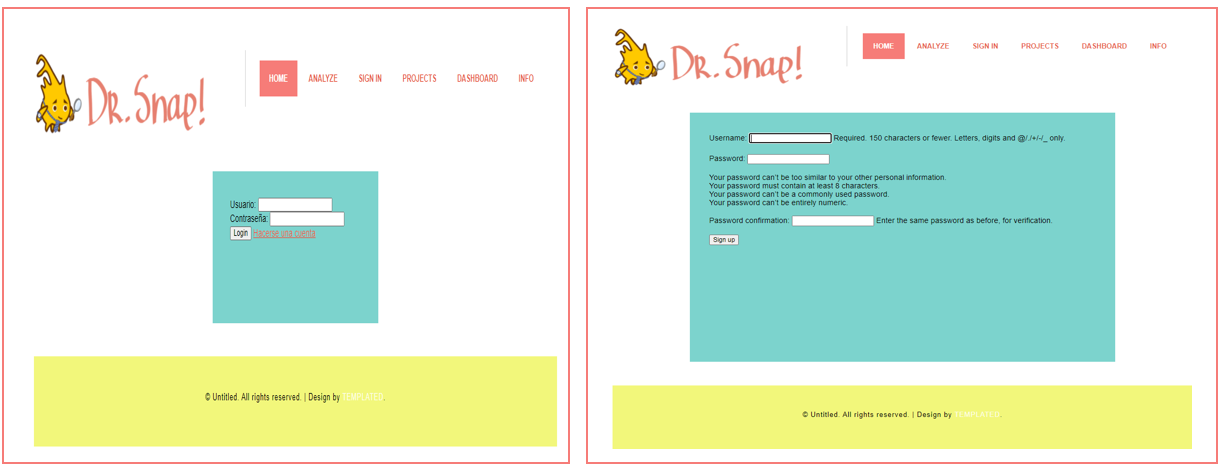
\includegraphics[scale=0.52]{img/sign.PNG}
            \caption{Inicio de sesión y registro en Dr. Snap!}
            \label{figura:sign}
    \end{figure}
\subsection{Modo profesor o estudiante}
Con la anterior opción se conseguía tener una base de datos con los proyectos analizados de los usuarios pero Dr. Snap! pretende ir más allá que analizar solo proyectos, como herramienta docente debe aportar distintas funcionalidades según el tipo de usuario que seas. Surge así, la distinción entre si eres estudiante o eres un profesor. Para ello se crea el modelo ``tipo'' que ya hemos mencionado donde se asocia el usuario con el tipo de usuario. Se implementa de forma que al darle al enlace de ``hacerse una cuenta'', mostrado en la figura~\ref{figura:sign}, te lleve al recurso /type-signup donde tienes dos formularios para elegir si eres estudiante o profesor. Una vez que seleccionas el tipo, la nueva entrada se guarda en la base de datos y se te redirige a la página de registro de la figura~\ref{figura:sign}. Esta funcionalidad queda reflejada en la figura~\ref{figura:tipo}. A continuación, se definen las prestaciones de casa modo:

\begin{itemize}
    \item Estudiante: tiene la opción de analizar sus proyectos y de ver gráficos con los proyectos analizados según los niveles obtenidos.
    \item Profesor: puede analizar proyectos propios o un conjunto de proyectos que deben estar comprimidos en formato ZIP. Se pensó que un profesor tendría varias clases y sería más sencillo analizar todos los proyectos de una clase subiéndolo como ZIP. Además, se da la opción de poder descargar en formato CSV la clase entera introduciendo el nombre del archivo ZIP que haya sido analizado previamente.
\end{itemize}

\begin{figure}[h]
\centering
            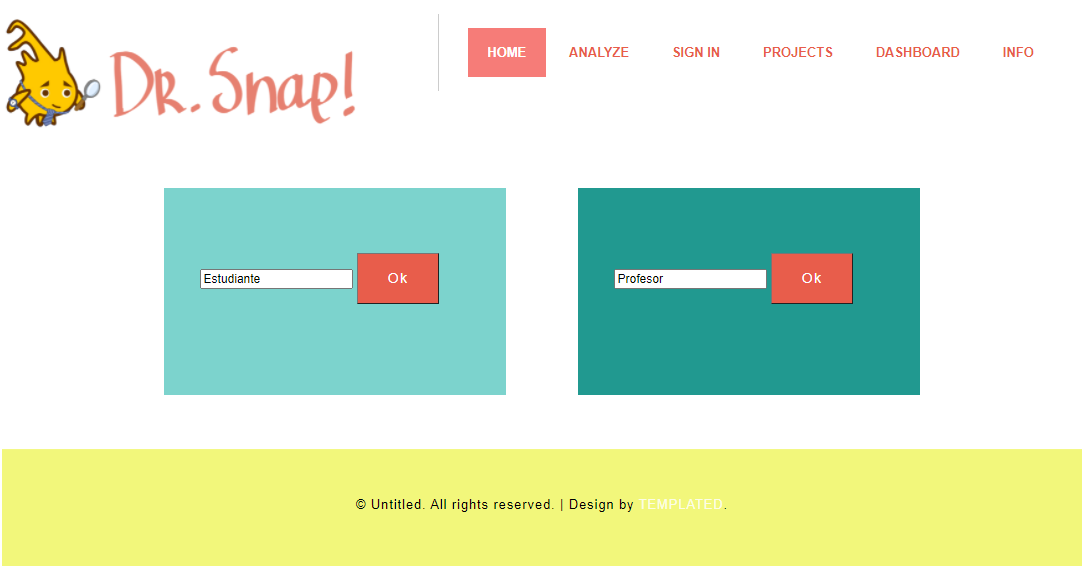
\includegraphics[scale=0.52]{img/tipo.PNG}
            \caption{Página para elegir el tipo de usuario en el proceso de registro en Dr. Snap!}
            \label{figura:tipo}
    \end{figure}
    
\subsection{Analizar ZIPs}
Para poder analizar un archivo ZIP debe ser subido primero a la aplicación por el usuario de tipo profesor. En la función de analizar proyectos, si estás logueado como profesor aparece un nuevo formulario en el que se ha implementado la posibilidad de importar un ZIP desde el ordenador. Para trabajar con el archivo comprimido hemos utilizado la librería ``FileSystemStorage'' importada de ``django.core.files.storage'' y con la librería ``zipFile''. De primeras, se dudó si trabajar con el archivo en local o en disco. Al final, me decanté por guardarlo en disco y trabajar con él ya que era menos complejo. En la figura~\ref{figura:zip} se muestra las opciones que ofrece la página analizar en caso de ser profesor. Los pasos para esta funcionalidad son los siguientes:
\begin{itemize}
    \item Guardar el archivo ZIP  en la carpeta llamada media, vista en la figura~\ref{figura:carpetas}. Esto se consigue con una función de ``FileSystemStorage'' llamada~\textit{fs.save()}.
    \item Quedarnos con la url donde se encuentra el ZIP con la función~\textit{fs.url()}.
    \item Descomprimir el ZIP con ``zipFile'' en una carpeta que se hace llamar: \textit{nombredeusuario\&nombredelarchivo } con la función~\textit{fs.urlextractall (password, path)}.
    \item Analizar cada proyecto calculando las puntuaciones y guardando los datos en la base de datos. En este punto es cuando se decide añadir un campo del modelo \textit{proyecto} que se llamó \textit{nombre\_zip} ya que de esta forma los proyectos que no pertecen a a ningún ZIP simplemente  este campo se pondría a NULL.
\end{itemize}
\begin{figure}[h]
\centering
            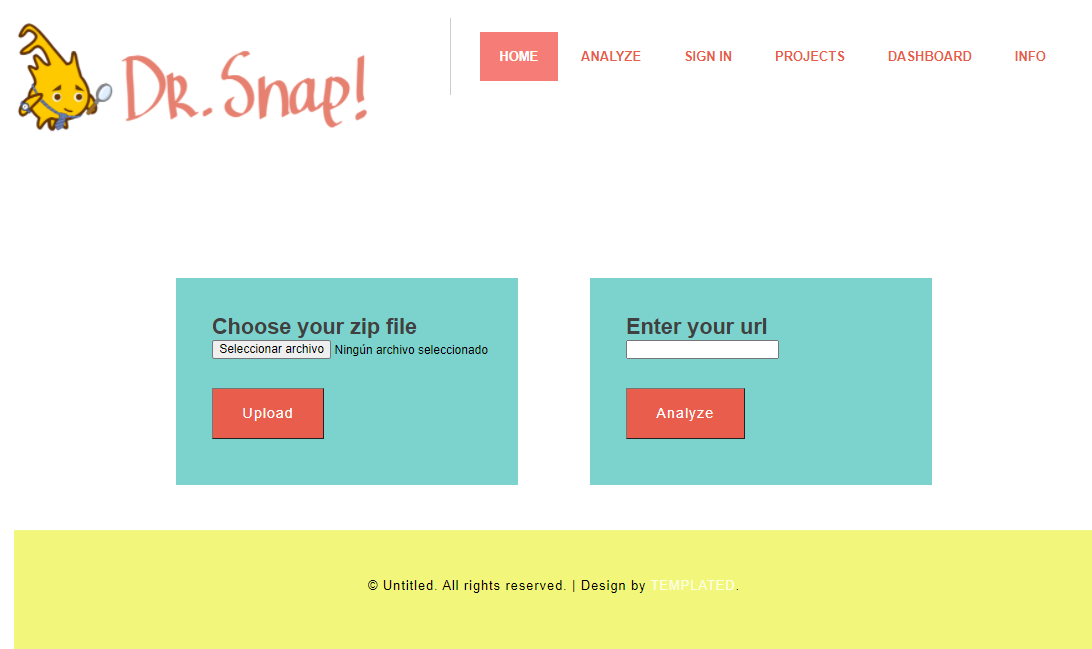
\includegraphics[scale=0.5]{img/zip.PNG}
            \caption{Formularios para subir un ZIP o analizar un proyecto en Dr. Snap!}
            \label{figura:zip}
    \end{figure}
\subsection{Dashboard}
       Los 3 dashboard que tenemos son los que enseñamos en la figura~\ref{figura:dshboard2} y otro más donde se compara los resultados de dos ZIPs que se hayan subido a la aplicación (figura~\ref{figura:dshboard}). Los datos que hemos cogido son los resultados de los proyectos que hay guardados en las cuentas de un estudiante o un profesor, es decir, han debido ser analizados previamente y guardados en la base de datos. ~Según el modo:
    \begin{itemize}
        \item Estudiante: sólo están disponibles los gráficos de la figura ~\ref{figura:dshboard2} y en ella se muestran los resultados de los proyectos que el alumno a analizado en Dr. Snap! en un diagrama de barras y en donut.\\
        \begin{figure}[h]
            \centering
            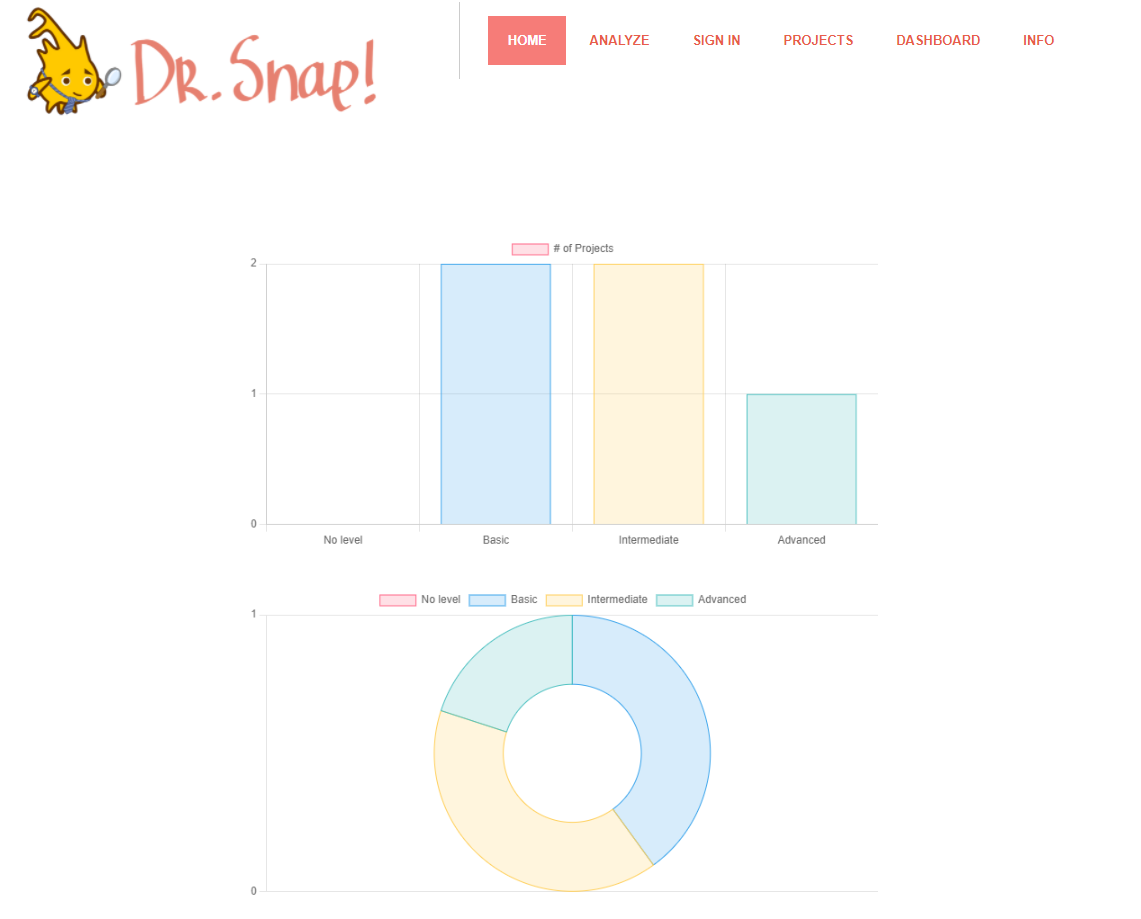
\includegraphics[scale=0.4]{img/dashboard.PNG}
            \caption{Dashboard de barra y de donut.}
            \label{figura:dshboard2}
        \end{figure}
        \item Profesor: además de los mencionados, se da la opción de ver los gráficos con los datos de una clase o incluso comparar un gráfico con dos clases diferentes (figura~\ref{figura:dshboard}). Cuando hablamos de clase se debe entender como un ZIP con los proyectos de los alumnos de una clase y que esta se ha analizado previamente gracias a la opción que damos de analizar ZIP.
         \begin{figure}[h]
            \centering
            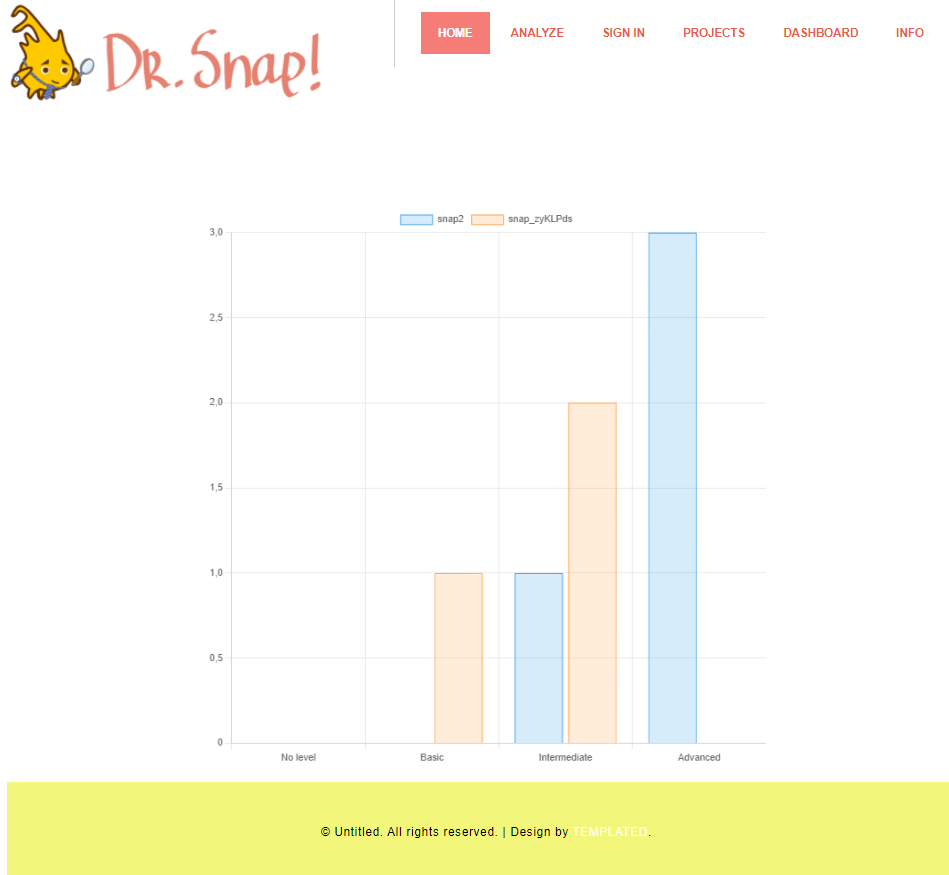
\includegraphics[scale=0.4]{img/comparar.PNG}
            \caption{Comparación de dos Zips}
            \label{figura:dshboard}
        \end{figure}
       
    \end{itemize}
    Para implementarlos hemos tenido que añadir un elemento ``canvas''~ de HTML que básicamente es un contenedor donde se dibujan los gráficos gracias a la librería de JavaScript ya mencionada ``Chart.js''. Una vez que dichos gráficos estaban implementados, se ha añadido la funcionalidad de que si haces click en una de las barras, por ejemplo en la azul de basic, te redirija a una tabla donde aparecen todos los proyectos de nivel básico. Esto ha requerido el aprendizaje de la programación basada en eventos ya que hacer click en la pantalla es un evento llamado onClick y hay que manejarlo para que distinga si estás pinchando dentro del elemento \textit{canvas}, si es fuera de las barras o porciones del donut y en caso de que sea dentro de ellas, distinguir qué nivel está pinchando.



%%%%%%%%%%%%%%%%%%%%%%%%%%%%%%%%%%%%%%%%%%%%%%%%%%%%%%%%%%%%%%%%%%%%%%%%%%%%%%%%
%%%%%%%%%%%%%%%%%%%%%%%%%%%%%%%%%%%%%%%%%%%%%%%%%%%%%%%%%%%%%%%%%%%%%%%%%%%%%%%%
% EXPERIMENTOS Y VALIDACIÓN %
%%%%%%%%%%%%%%%%%%%%%%%%%%%%%%%%%%%%%%%%%%%%%%%%%%%%%%%%%%%%%%%%%%%%%%%%%%%%%%%%

\cleardoublepage
\chapter{Experimentos y validación}

Este capítulo se introdujo como requisito en 2019. 
Describe los experimentos y casos de test que tuviste que implementar para validar tus resultados. 
Incluye también los resultados de validación que permiten afirmar que tus resultados son correctos. 


%%%%%%%%%%%%%%%%%%%%%%%%%%%%%%%%%%%%%%%%%%%%%%%%%%%%%%%%%%%%%%%%%%%%%%%%%%%%%%%%
%%%%%%%%%%%%%%%%%%%%%%%%%%%%%%%%%%%%%%%%%%%%%%%%%%%%%%%%%%%%%%%%%%%%%%%%%%%%%%%%
% RESULTADOS %
%%%%%%%%%%%%%%%%%%%%%%%%%%%%%%%%%%%%%%%%%%%%%%%%%%%%%%%%%%%%%%%%%%%%%%%%%%%%%%%%

\cleardoublepage
\chapter{Resultados}

En este capítulo se incluyen los resultados de tu trabajo fin de grado.

Si es una herramienta de análisis lo que has realizado, aquí puedes poner ejemplos de haberla utilizado para que se vea su utilidad.


%%%%%%%%%%%%%%%%%%%%%%%%%%%%%%%%%%%%%%%%%%%%%%%%%%%%%%%%%%%%%%%%%%%%%%%%%%%%%%%%
%%%%%%%%%%%%%%%%%%%%%%%%%%%%%%%%%%%%%%%%%%%%%%%%%%%%%%%%%%%%%%%%%%%%%%%%%%%%%%%%
% CONCLUSIONES %
%%%%%%%%%%%%%%%%%%%%%%%%%%%%%%%%%%%%%%%%%%%%%%%%%%%%%%%%%%%%%%%%%%%%%%%%%%%%%%%%

\cleardoublepage
\chapter{Conclusiones}
\label{chap:conclusiones}


\section{Consecución de objetivos}
\label{sec:consecucion-objetivos}

Esta sección es la sección espejo de las dos primeras del capítulo de objetivos, donde se planteaba el objetivo general y se elaboraban los específicos.

Es aquí donde hay que debatir qué se ha conseguido y qué no. 
Cuando algo no se ha conseguido, se ha de justificar, en términos de qué problemas se han encontrado y qué medidas se han tomado para mitigar esos problemas.

Y si has llegado hasta aquí, siempre es bueno pasarle el corrector ortográfico, que las erratas quedan fatal en la memoria final.
Para eso, en Linux tenemos aspell, que se ejecuta de la siguiente manera desde la línea de \emph{shell}:

\begin{verbatim}
  aspell --lang=es_ES -c memoria.tex
\end{verbatim}

\section{Aplicación de lo aprendido}
\label{sec:aplicacion}

Aquí viene lo que has aprendido durante el Grado/Máster y que has aplicado en el TFG/TFM. Una buena idea es poner las asignaturas más relacionadas y comentar en un párrafo los conocimientos y habilidades puestos en práctica.

\begin{enumerate}
  \item a
  \item b
\end{enumerate}


\section{Lecciones aprendidas}
\label{sec:lecciones_aprendidas}

Aquí viene lo que has aprendido en el Trabajo Fin de Grado/Máster.

\begin{enumerate}
  \item Aquí viene uno.
  \item Aquí viene otro.
\end{enumerate}


\section{Trabajos futuros}
\label{sec:trabajos_futuros}

Ningún proyecto ni software se termina, así que aquí vienen ideas y funcionalidades que estaría bien tener implementadas en el futuro.

Es un apartado que sirve para dar ideas de cara a futuros TFGs/TFMs.


%%%%%%%%%%%%%%%%%%%%%%%%%%%%%%%%%%%%%%%%%%%%%%%%%%%%%%%%%%%%%%%%%%%%%%%%%%%%%%%%
%%%%%%%%%%%%%%%%%%%%%%%%%%%%%%%%%%%%%%%%%%%%%%%%%%%%%%%%%%%%%%%%%%%%%%%%%%%%%%%%
% APÉNDICE(S) %
%%%%%%%%%%%%%%%%%%%%%%%%%%%%%%%%%%%%%%%%%%%%%%%%%%%%%%%%%%%%%%%%%%%%%%%%%%%%%%%%

\cleardoublepage
\appendix
\chapter{Manual de usuario}
\label{app:manual}

Esto es un apéndice.
Si has creado una aplicación, siempre viene bien tener un manual de usuario.
Pues ponlo aquí.

%%%%%%%%%%%%%%%%%%%%%%%%%%%%%%%%%%%%%%%%%%%%%%%%%%%%%%%%%%%%%%%%%%%%%%%%%%%%%%%%
%%%%%%%%%%%%%%%%%%%%%%%%%%%%%%%%%%%%%%%%%%%%%%%%%%%%%%%%%%%%%%%%%%%%%%%%%%%%%%%%
% BIBLIOGRAFIA %
%%%%%%%%%%%%%%%%%%%%%%%%%%%%%%%%%%%%%%%%%%%%%%%%%%%%%%%%%%%%%%%%%%%%%%%%%%%%%%%%

\cleardoublepage

% Las siguientes dos instrucciones es todo lo que necesitas
% para incluir las citas en la memoria
\bibliographystyle{abbrv}
\bibliography{memoria}  % memoria.bib es el nombre del fichero que contiene
% las referencias bibliográficas. Abre ese fichero y mira el formato que tiene,
% que se conoce como BibTeX. Hay muchos sitios que exportan referencias en
% formato BibTeX. Prueba a buscar en http://scholar.google.com por referencias
% y verás que lo puedes hacer de manera sencilla.
% Más información: 
% http://texblog.org/2014/04/22/using-google-scholar-to-download-bibtex-citations/

\end{document}
